\documentclass[hidelinks,onefignum,onetabnum,final]{siamart220329}  % for arxiv
%\documentclass[review,hidelinks,onefignum,onetabnum,final]{siamart220329}  % for submission

\usepackage{amsfonts,yhmath}
\usepackage{graphicx}
\usepackage{epstopdf}
\ifpdf
  \DeclareGraphicsExtensions{.eps,.pdf,.png,.jpg}
\else
  \DeclareGraphicsExtensions{.eps}
\fi

% Used for creating new theorem and remark environments
\newsiamremark{remark}{Remark}
\newsiamthm{claim}{Claim}
\newsiamremark{example}{Example}

\newcommand{\newindthm}[2]{
  \theoremstyle{plain}
  \theoremheaderfont{\normalfont\sc}
  \theorembodyfont{\normalfont\itshape}
  \theoremseparator{.}
  \theoremsymbol{}
  \newtheorem{#1}{#2}
}
\newindthm{conjecture}{Conjecture}
\renewcommand{\theconjecture}{\Alph{conjecture}}

\newcommand{\newindthmstar}[2]{
  \theoremstyle{plain}
  \theoremheaderfont{\normalfont\sc}
  \theorembodyfont{\normalfont\itshape}
  \theoremseparator{.}
  \theoremsymbol{}
  \newtheorem*{#1}{#2}
}
\newindthmstar{assumptions}{Standard Assumptions}

\usepackage{amsopn}
\DeclareMathOperator{\diag}{diag}

\usepackage{bm,bbm,empheq,verbatim,fancyvrb,amssymb}
\usepackage{booktabs,multirow,xspace}
\usepackage{pifont}

\usepackage{tikz}
\usetikzlibrary{decorations.pathreplacing}
\usetikzlibrary{graphs,quotes}

\newcommand{\eps}{\epsilon}
\newcommand{\RR}{\mathbb{R}}

\newcommand{\grad}{\nabla}
\newcommand{\Div}{\nabla\cdot}

\newcommand{\bbf}{\mathbf{f}}
\newcommand{\bg}{\mathbf{g}}
\newcommand{\bn}{\mathbf{n}}
\newcommand{\bu}{\mathbf{u}}
\newcommand{\bv}{\mathbf{v}}
\newcommand{\bw}{\mathbf{w}}
\newcommand{\bx}{\mathbf{x}}
\newcommand{\bz}{\mathbf{z}}

\newcommand{\bX}{\mathbf{X}}

\newcommand{\bzero}{\bm{0}}

\newcommand{\btau}{\bm{\tau}}

\newcommand{\cB}{\mathcal{B}}
\newcommand{\cH}{\mathcal{H}}
\newcommand{\cK}{\mathcal{K}}
\newcommand{\cQ}{\mathcal{Q}}
\newcommand{\cV}{\mathcal{V}}
\newcommand{\cX}{\mathcal{X}}

\newcommand{\hcK}{\widehat{\cK}}

\newcommand{\nn}{{\text{\textnormal{n}}}}
\newcommand{\pp}{{\text{\textnormal{p}}}}
\newcommand{\qq}{{\text{\textnormal{q}}}}
\newcommand{\rr}{{\text{\textnormal{r}}}}

\newcommand{\ip}[2]{\left<#1,#2\right>}

\newcommand{\XX}{\ding{55}}

\newcommand{\dx}{\, \mathrm{d}x}

\newcommand{\rhoi}{\rho_{\text{i}}}

\DeclareMathOperator*{\argmin}{arg\,min}
\DeclareMathOperator*{\Hull}{Hull}

\newcommand{\Vdiv}{\cV_{\text{\textnormal{div}}}}

\newcommand{\CA}{C_\text{\textnormal{A}}}

% running headers and PDF metadata
\headers{Glacier geometry evolution under Stokes dynamics}{E. Bueler}

\title{Glacier geometry evolution under Stokes dynamics}

\author{Ed Bueler\thanks{Department of Mathematics and Statistics, University of Alaska Fairbanks, USA (\email{elbueler@alaska.edu}).}}


\begin{document}
\maketitle

\begin{abstract}
The primary data which determine the evolution of glaciation are the bedrock elevation and surface mass balance functions.  From this data the glacier's geometry solves a free-boundary problem over a set of admissible surface elevation functions; a surface is admissible if it is above the bedrock topography, equivalently if the ice thickness is nonnegative.  For an implicit time step, this free-boundary problem can be posed in weak form as a variational inequality over a fixed map-plane region.  After some preparatory theory, recalling and expanding upon what is known about the glaciological Stokes problem, we conjecture that, in the case of Stokes dynamics, the continuous-space problems at each implicit time step are well-posed.  This conjecture is supported by certain numerical evidence.  We then prove a general theorem which estimates the error made by a finite element approximation of a variational inequality problem over a Banach space.  The provided estimate is a sum of errors of different types, mostly specific to variational inequalities.  When specialized to the glacier case the terms in the error estimate can be physically-interpreted.  Practical approaches to bound and/or reduce these errors are then proposed.
\end{abstract}

% REQUIRED
\begin{keywords}
error bounds, finite element methods, glaciers, ice flow, variational inequalities
\end{keywords}

% REQUIRED
%\begin{MSCcodes}
%FIXME
%\end{MSCcodes}


\section{Introduction} \label{sec:intro}

Glacier and ice sheet simulations typically model the ice as a free-surface layer of very-viscous, incompressible, and non-Newtonian fluid \cite{GreveBlatter2009,SchoofHewitt2013}.  For simplicity we will only consider such simulations of glaciers on land, without floating portions.  Note that an ``ice sheet'' is simply a continent-scale glacier.

The two essential types of input data into such simulations are the bedrock elevation, which is assumed here to be constant in time, and the time-dependent surface mass balance rate (SMB; it is also called the climatic mass balance rate \cite{Cogleyetal2011}).  By definition, the SMB is the difference between the vertically-accumulating snow and the loss of (liquid) water, through runoff, at the upper surface of the glacier \cite{Cogleyetal2011}.  It is positive in areas of snow accumulation, and it is often provided only through annual averages.  Note that elevations are measured here in meters, while SMB is measured in ice-equivalent units of meters per second.

Thus a glacier simulation takes, as inputs, at least these data: the bedrock topography, a (generally) time-dependent climate, and an initial geometry.  It produces the glacier's evolving geometry and flow velocity, the output fields of primary scientific value.  Note that additional complications are common in comprehensive ice sheet models \cite{SchoofHewitt2013,Winkelmannetal2011}.  For example, the internal energy \cite{Aschwandenetal2012} or temperature of the ice may be tracked, and/or any liquid water within the ice matrix and at ice surfaces.  However, here we only consider conservation of mass and momentum, but not of energy, and liquid water plays no role.  Furthermore we will assume zero velocity, i.e.~a non-sliding and non-penetrating condition, at the base of the ice.  On the other hand, we will not make the shallowness assumptions which are common in comprehensive models.

The glacier's geometry is parameterized by either the (upper) surface elevation or the ice thickness.  However, the computed flow velocity is only defined at those locations and times where ice is present, namely on an evolving 3D domain between the bedrock and surface elevations.  Furthermore, at a time and map-plane location where a glacier exists the surface elevation must exceed the bedrock elevation, equivalently the ice thickness must be positive.  That is, the glacier's geometry must satisfy an inequality to be admissible.

To expand upon this inequality we start with the notation sketched in Figure \ref{fig:stokesdomain}.  Let $\Omega \subset \RR^2$ be a fixed portion of land, with map-plane coordinates $x=(x_1,x_2)\in\Omega$.  All time-dependent quantities are assumed to be defined for $t\in [0,T]$ for some given $T>0$.  On $\Omega$ assume that we are given, as data, a real, continuous, and time-independent bed elevation function $b(x)$, and a real, continuous SMB function $a(t,x)$, generally taking both signs.  In areas where $a>0$ (accumulation; downward arrows in Figure \ref{fig:stokesdomain}), a glacier will exist.  If $a<0$ (upward arrows) then either a glacier exists with an ablating surface, or no glacier exists.  Determining which situation applies at a given point $t,x$ requires solving free-boundary problems like those considered in this paper.

\begin{figure}[ht]
\centering
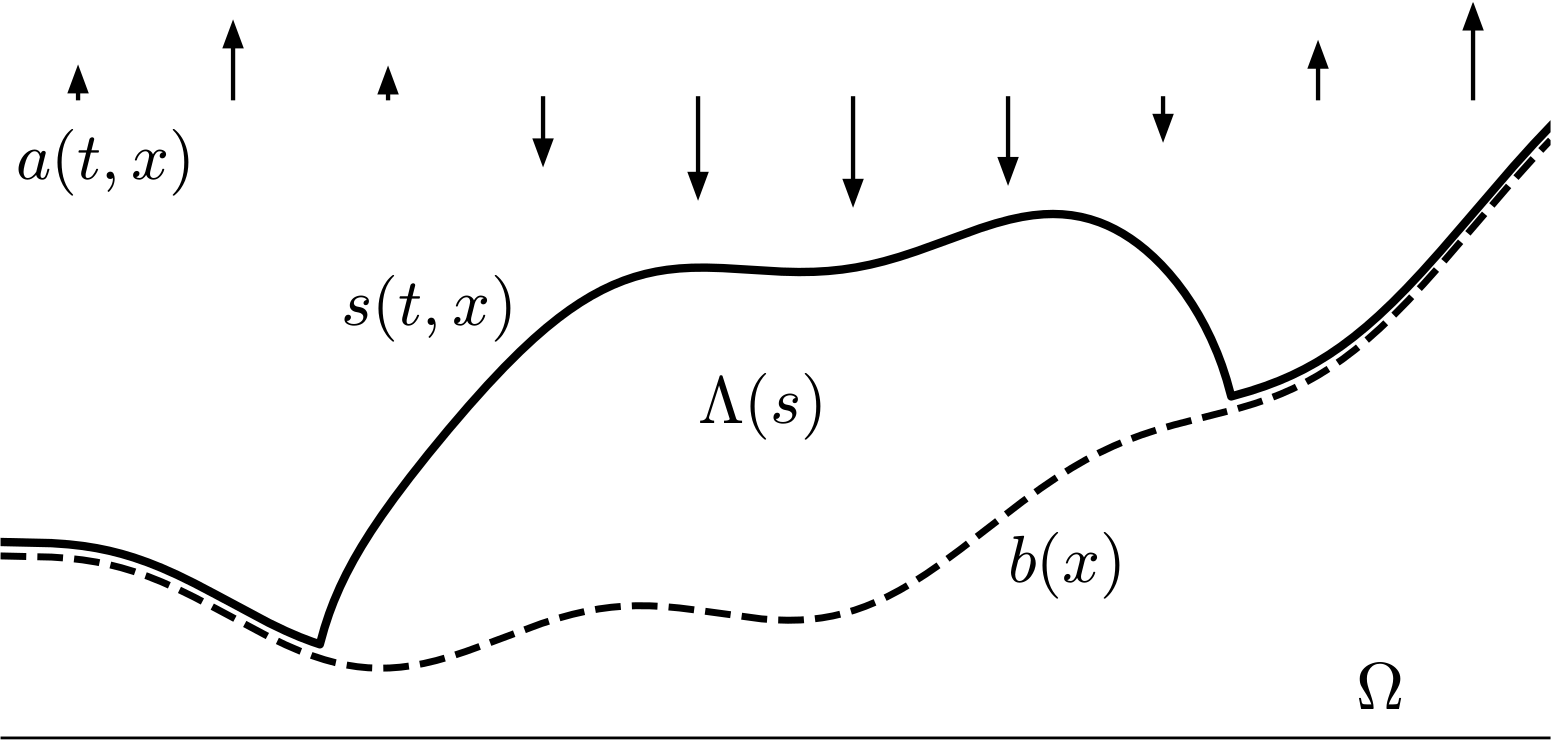
\includegraphics[width=0.65\textwidth]{genfigs/stokesdomain.pdf}
\caption{Glacier notation used in this paper.}
\label{fig:stokesdomain}
\end{figure}

Let $s(t,x)$ be the (solution) ice surface elevation.  We will regard this as defined for all $x\in\Omega$, and subject to the constraint that the surface $z=s$ must be at or above the bedrock ($s \ge b$), and in regions with no ice we set $s=b$.  The solution ice velocity $\bu(t,x,z)$ and pressure $p(t,x,z)$ are then defined only on the 3D domain
\begin{equation}
\Lambda(t) = \left\{(x,z)\,:\,b(x) < z < s(t,x)\right\} \subset \Omega \times \RR. \label{eq:icydomain}
\end{equation}
This aspect of glacier modeling deserves emphasis:  The time-dependent 3D domain $\Lambda(t)$, on which the solution velocity and pressure are meaningful, is determined by the evolving surface elevation $s(t,x)$, which is itself part of the model solution.

The surface trace of the ice velocity will be of importance.  We extend it by zero so that it is defined everywhere in $\Omega$.  Let
\begin{equation}
\bu|_s(t,x) = \begin{cases} \bu(t,x,s(t,x)), & s(t,x)>b(t,x) \\
                            \bzero, & \text{otherwise} .\end{cases} \label{eq:defineus}
\end{equation}
Compare flux extension by zero in \cite{SchoofHewitt2013}.  Definition \eqref{eq:defineus} will be reconsidered later in a precise Sobolev space context.

Let $\bn_s = \left<-\grad s,1\right>$ be an un-normalized and upward surface normal vector.  (This is assumed well-defined for the purposes of this Introduction; compare Section \ref{sec:model}.)  Then an infinite-dimensional nonlinear complementarity problem (NCP) \cite{Bueler2021conservation,FacchineiPang2003,SchoofHewitt2013} applies almost everywhere in $[0,T]\times \Omega$:
\begin{subequations}
\label{eq:ncp}
\begin{align}
s - b &\ge 0 \\
\frac{\partial s}{\partial t} - \bu|_s \cdot \bn_s - a &\ge 0 \\
(s - b) \left(\frac{\partial s}{\partial t} - \bu|_s \cdot \bn_s - a\right) &= 0
\end{align}
\end{subequations}
This strong form NCP statement will be reformulated as a variational inequality (VI; \cite{KinderlehrerStampacchia1980}), a weak form, in Section \ref{sec:model}.  System \eqref{eq:ncp} says that either a location is ice free ($s-b=0$), where the climate is, necessarily, locally ablating ($a\le 0$), or that the surface kinematical equation (SKE) holds:
\begin{equation}
\frac{\partial s}{\partial t} - \bu|_s \cdot \bn_s - a = 0.  \label{eq:ske}
\end{equation}
SKE \eqref{eq:ske} says that the (non-material) surface of the ice moves vertically according to the sum of the SME and a component of the ice velocity at the surface \cite{SchoofHewitt2013}.  Equation \eqref{eq:ske} is a statement of mass conservation at a non-material surface \cite{Aschwandenetal2012}, sometimes called the free-surface equation \cite{LofgrenAhlkronaHelanow2022} or the kinematic boundary condition\footnote{Note that equation \eqref{eq:ske} is not a boundary condition of any identifiable PDE problem.} \cite{GreveBlatter2009}.

In the current paper the SMB $a$ is necessarily assumed to be defined everywhere in $\Omega$, regardless of whether a glacier is present or not.  At an ice-free location the SMB value can be modeled using precipitation and an energy balance \cite{GreveBlatter2009}, for instance by hypothesizing an ice or snow surface and then computing the balance of snow accumulation minus the total ablation from the energy available for melt.  Because a simulated glacier needs to be able to advance into unglaciated locations, the SMB there should have the value which a glacier surface would experience at that time and location.

The continuum models considered in this paper conserve mass and momentum.   The (standard) non-shallow ice dynamics model used here is a non-sliding (e.g.~frozen) base, isothermal, shear-thinning (non-Newtonian), and incompressible Stokes problem \cite{GreveBlatter2009,JouvetRappaz2011,SchoofHewitt2013}, applied over the domain $\Lambda(t)$ defined in \eqref{eq:icydomain}.  Let $\Gamma_s(t) \subset \partial \Lambda(t)$ be the upper surface $z=s$ and $\Gamma_b(t) \subset \partial \Lambda(t)$ be the base $z=b$.  The possibility of cliffs at the ice margin is neglected, so $\partial \Lambda(t) = \overline{\Gamma_s(t)} \cup \overline{\Gamma_b(t)}$ is assumed to hold at any time.

To state the shear-thinning (Glen's) flow law, let $D\bu=(\grad \bu + \grad \bu^{\top})/2$ denote the strain rate tensor, with Frobenius norm $|D\bu| = (D\bu:D\bu)^{1/2} = \left((D\bu)_{ij} (D\bu)_{ij}\right)^{1/2}$.  The effective ice (dynamic) viscosity \cite{GreveBlatter2009} is given by a regularized formula
\begin{equation}
\nu(D\bu) = \nu_\pp \left(|D\bu|^2 + \eps\right)^{(\pp-2)/2} \label{eq:glen}
\end{equation}
The exponent $1 < \pp \le 2$, often written $\pp=(1/\nn)+1$, is approximately 4/3 in practice because $\nn\approx 3$ \cite{GreveBlatter2009}.  The coefficient $\nu_\pp>0$ has $\pp$-dependent units, but $\nu(D\bu)$ has SI units $\text{kg}\,\text{m}^{-1}\,\text{s}^{-1}$.  The values of $\nn$ and $\nu_\pp$ can be determined from measured properties of ice \cite{GoldsbyKohlstedt2001,GreveBlatter2009}, including temperature, but both are assumed to be constant (isothermal) here.  Note that $\pp=2$ yields a Newtonian fluid with constant viscosity, while for $\pp < 2$ the $\eps>0$ regularization implies that $\nu(D\bu)$ is bounded above.

Assume that the density of ice $\rhoi$ and the acceleration of gravity $\bg$ are constant.  At each time $t$ the modeled glacier has velocity and pressure solving the following 3D fluid equations:
\begin{subequations}
\label{eq:stokes}
\begin{align}
- \nabla \cdot \left(2 \nu(D\bu)\, D\bu\right) + \nabla p &= \rhoi \bg && \text{within $\Lambda(t)$} \\
\nabla \cdot \bu &= 0 && \qquad \text{''} \label{eq:stokes:incomp} \\
\left(2 \nu(D\bu) D\bu - pI\right) \bn_s &= \bzero && \text{on $\Gamma_s(t)$}\label{eq:stokes:stressfreesurface} \\
\bu  &= \bzero && \text{on $\Gamma_b(t)$}
\end{align}
\end{subequations}
Note that boundary condition \eqref{eq:stokes:stressfreesurface} says that the sub-aerial upper surface is stress free; this should not be confused with the SKE \eqref{eq:ske}.

In summary at this point, a glacier simulation is an evolving free-surface flow, subject to a signed climate that can add or remove ice, coupled to a nonlinear Stokes problem which must be solved within an evolving, 3D icy domain.  A well-posed initial/boundary value problem for \eqref{eq:icydomain}--\eqref{eq:stokes} will require data $b(x),a(t,x)$ plus an initial surface elevation $s(0,x)$.  The solution variables are $s(t,x)$, $\bu(t,x,z)$, and $p(t,x,z)$, with $s$ defined everywhere over $[0,T]\times \Omega$, but subject to $s \ge b$, and with $\bu,p$ defined on $\Lambda(t)$ for each $t$.  The surface elevation $s$ and surface velocity $\bu|_s$ are linked by the kinematical NCP \eqref{eq:ncp}, which is the only place that a time derivative appears in the model equations.  Because the flow is very viscous \cite{Acheson1990}, the Stokes sub-model \eqref{eq:glen}--\eqref{eq:stokes} acts as an instantaneous ``algebraic'' constraint on the evolution statement in \eqref{eq:ncp}.  The coupled, infinite-dimensional problem of determining the evolving geometry of a glacier, namely system \eqref{eq:icydomain}--\eqref{eq:stokes}, is therefore both a differential algebraic equation (DAE) system \cite{AscherPetzold1998,LofgrenAhlkronaHelanow2022} and an NCP.

As already noted, one may choose to parameterize the glacier geometry by either surface elevation or thickness.  While essentially equivalent in the (continuum) problem, formulations using these different functions have different character when the bedrock is realistically rough.  Specifically, when applying the abstract estimate of Section \ref{sec:abstractestimate}, surface elevation $s$ will be preferred because of the flow-caused smoothing effect illustrated in Figure \ref{fig:giscross}.  That is, we observe that for land-based glaciers $s(t,x)$ is smoother in $x$ than the thickness $H(t,x) = s(t,x)-b(x)$ because the latter ``inherits'' the lower regularity of the (typically) eroded and/or faulted bedrock topography $b(x)$.

\begin{figure}
\begin{minipage}[t]{0.85\textwidth}
\vspace{0pt}
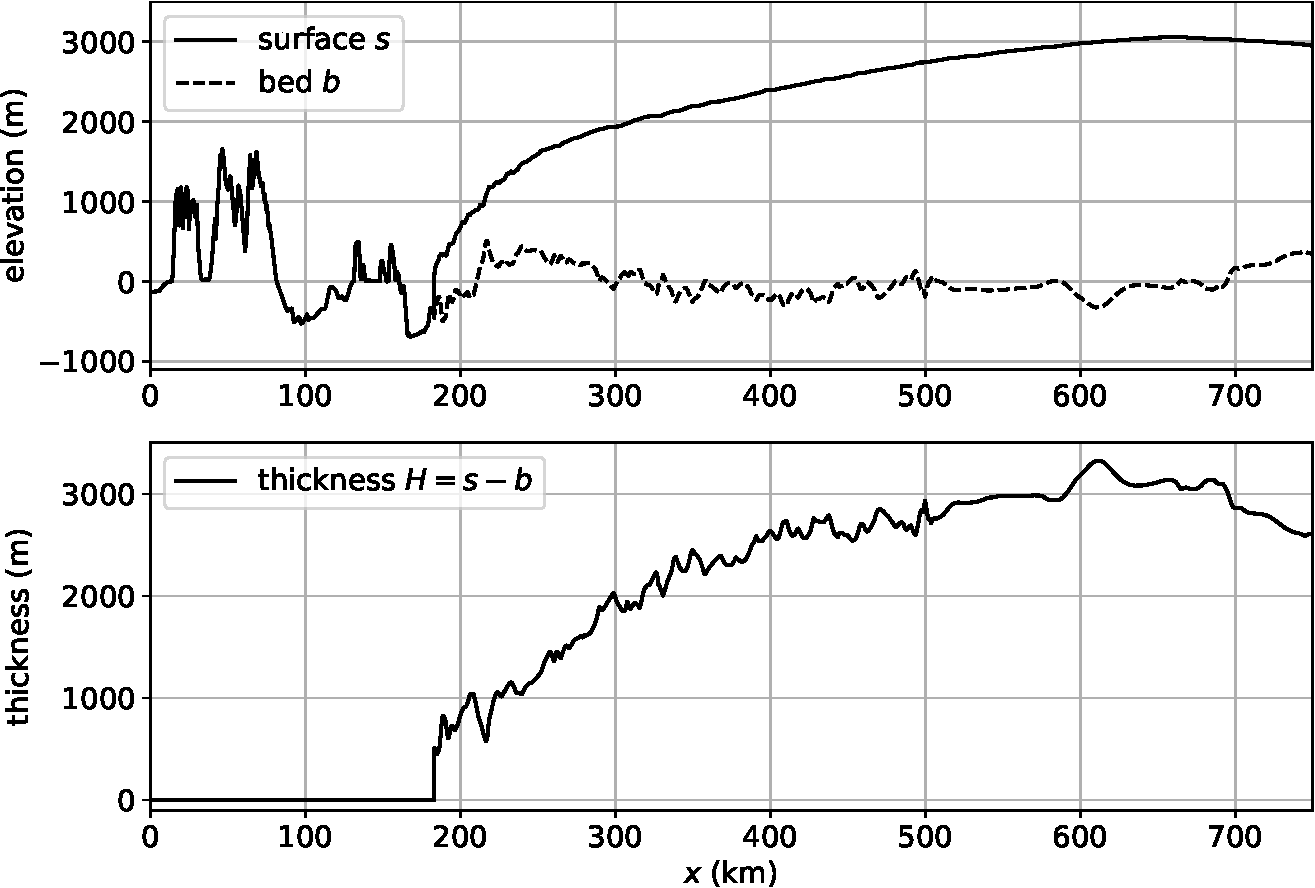
\includegraphics[width=\textwidth]{genfigs/giscross.pdf}
\end{minipage}
\,
\begin{minipage}[t]{0.13\textwidth}
\vspace{10pt}
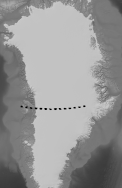
\includegraphics[width=\textwidth]{genfigs/gis/gris-profile-gray.png}
\end{minipage}
\caption{A cross-section of the Greenland ice sheet at $70^\circ$N latitude (see inset).  While the ice surface $s$ is relatively smooth because of ice flow (top), the bedrock elevation $b$ is much rougher.  The corresponding ice thickness $H = s-b$ (bottom), though a valid geometry parameterization, inherits the low regularity of $b$.  (Data from \cite{Morlighemetal2017} and A.~Aschwanden, personal communication.)}
\label{fig:giscross}
\end{figure}

Glacier simulations are commonly formulated using a finite element (FE) method for the Stokes sub-problem \cite{IsaacStadlerGhattas2015,Jouvetetal2008,Pattynetal2008}, or for a shallow approximation thereof.  However, to the author's knowledge all existing non-shallow (Stokes) evolution models use a explicit time-stepping scheme for the geometry, for example as in \cite{Jouvetetal2008} or \cite{LofgrenAhlkronaHelanow2022}, with the one exception of the exploratory model in reference \cite{WirbelJarosch2020}.  In the current paper we consider implicit time steps, for the theoretical reasons which are addressed here.  One can also make a case for implicit time-stepping based on simulation performance concerns; see \cite{Bueler2023}.

FIXME: state backward Euler step SKE \eqref{eq:be:ske} here, to commit to implicit

FIXME: WHAT WE ACCOMPLISH

This paper is organized as follows.  Section \ref{sec:stokes} recalls the existing theory of the Glen-law Stokes problem on a fixed domain, but we add an apparently-new bound on the surface trace of the velocity solution (Corollary \ref{cor:surfacetracebound}).  In Section \ref{sec:model} we discretize the time derivative and then reformulate the coupled problem \eqref{eq:icydomain}--\eqref{eq:stokes} as a VI weak form for an implicit (backward Euler) time step.  The key coupling term in this problem is the surface motion portion (i.e.~$\bu|_s\cdot \bn_s$) of the SKE \eqref{eq:ske}, for which we provide a quantitative bound (Lemma \ref{lem:philipschitz}) over a Sobolev space of surface elevation functions.  However, this bound is subject to a conjecture that the surface trace of velocity is Lipschitz continuous with respect to surface elevation.  Well-posedness for each implicit time-step problem is considered in Section \ref{sec:theory}, including a second conjecture on the coercivity of the surface motion term.  Certain physical and modeling ideas are discussed here, as context needed to understand the latter conjecture.  At this point we have in hand a mathematically-precise, time-discretized continuum model, though one with only conjectural well-posedness; see Theorem \ref{thm:stepwellposed}.  This continuum model, precisely stated here for what we believe is the first time, is one which can be approximated by a finite element (FE) method.  In Section \ref{sec:abstractestimate} we prove an abstract FE error estimate, namely Theorem \ref{thm:abstractestimate}, and its corollaries, for general VI problems involving fully-nonlinear operators on Banach spaces.  This new estimate, which makes coercive and Lipshitz assumptions, extends the classical case by Falk \cite{Falk1974} for bilinear forms.  [FIXME: rewrite needed from here] In Section \ref{sec:application} we apply the estimate to the glacier model.  The distinctive character of non-sliding land-based glaciers, in terms of how they respond to climate (mass balance) perturbations, and how they stagnate as ice thickness approaches zero, implies that certain terms in the error estimate are small.  Computable geometry error upper bounds follow.  These estimates are demonstrated in Section \ref{sec:demo} on an idealized, but non-trivial, glacier simulation implemented in Firedrake \cite{Hametal2023}.


\section{The surface velocity from a glacier Stokes problem} \label{sec:stokes}

In this Section we consider the weak form of the non-sliding, isothermal, and Glen-law Stokes sub-model \eqref{eq:glen}--\eqref{eq:stokes}.  This sub-model is applied on a fixed 3D domain $\Lambda = \Lambda(t)$, defined by \eqref{eq:icydomain}, at a fixed time $t$, and it computes the surface velocity field $\bu|_s$ which appears in NCP \eqref{eq:ncp}.  Note that the weak form of \eqref{eq:ncp} will be presented in Section \ref{sec:model} below.

Suitable function spaces for Stokes problem \eqref{eq:glen}--\eqref{eq:stokes} are well-known so long as the domain $\Lambda$ is sufficiently regular.  We will assume that the ice base $\Gamma_b\subset\partial \Lambda$, on which a Dirichlet condition $\bu=\bzero$ holds, has positive measure, and that the remaining Neumann boundary $\Gamma_s = \partial \Lambda \setminus \overline{\Gamma_b}$ is sufficiently-smooth so that a zero normal stress condition can be applied.

Let $1 < \pp \le 2$.  (Recall that $\pp=(1/\nn)+1\approx 4/3$ in viscosity formula \eqref{eq:glen}.)  The Sobolev space \cite{Evans2010} of real-valued functions with $\pp$th-power integrable first derivatives is denoted $W^{1,\pp}(\Lambda)$.  Let
\begin{equation}
\cV = W_b^{1,\pp}(\Lambda; \RR^3) \label{eq:defineV}
\end{equation}
denote the corresponding space of vector-valued functions with value (trace) zero along $\Gamma_b$.  Let $[L]>0$ be a representative \emph{horizontal} glacier dimension.  We define the norm on $\cV$ by
\begin{equation}
\|\bv\|_{\cV} = \left(\int_\Lambda |\bv|^\pp\,dx\,dz + [L]^\pp \int_\Lambda |\grad\bv|^\pp\,dx\,dz\right)^{1/\pp}. \label{eq:vnorm}
\end{equation}
Here $dx\,dz = dx_1\,dx_2\,dz$ is the 3D volume element, which will be suppressed from now on in integrals over $\Lambda$.  Note that $|\bv|$ denotes the Euclidean norm of $\bv\in\RR^3$ and $|\grad\bv|=\left((\grad\bv)_{ij} (\grad\bv)_{ij}\right)^{1/2}$ is the Frobenius norm of $\grad\bv\in\RR^{3\times 3}$.  Remark 1.2.1 in \cite{BoffiBrezziFortin2013} explains the length scaling in \eqref{eq:vnorm}, such that $\|\bv\|_{\cV}$ has consistent units.

Let $\cQ=L^{\pp'}(\Lambda)$ where $\pp'=\pp/(\pp-1)\approx 4$ is the conjugate exponent.  Define
\begin{equation}
\mathcal{M} = \cV \times \cQ \label{eq:glenstokes:mixedspace}
\end{equation}
as the space of admissible velocity and pressure pairs.  For $(\bu,p) \in \mathcal{M}$ define
\begin{equation}
F_\Lambda(\bu,p)[\bv,q] = \int_\Lambda 2 \nu(D\bu) D\bu : D\bv - p \Div\bv - (\Div\bu) q - \rhoi \bg \cdot \bv. \label{eq:glenstokes:fcnl}
\end{equation}
The (mixed) weak form of the Stokes sub-model seeks the solution $(\bu,p)$ satisfying
\begin{equation}
F_\Lambda(\bu,p)[\bv,q] = 0 \qquad \text{for all } (\bv,q) \in \mathcal{M}. \label{eq:glenstokes:weak}
\end{equation}

Jouvet and Rappaz \cite{JouvetRappaz2011} have proven that problem \eqref{eq:glenstokes:weak} is well-posed if the Neumann portion of $\partial\Lambda$ is $C^1$.  Their proof uses the equivalence of \eqref{eq:glenstokes:weak} and the minimization of a convex and coercive functional over the divergence-free subspace $\Vdiv = \{\bv\in\cV\,:\,\Div\bv=0\}$.  Our regularization in Glen law \eqref{eq:glen} differs from that in \cite{JouvetRappaz2011}, but the necessary modifications are addressed in \cite{IsaacStadlerGhattas2015}.  Note that if the weak solution is sufficiently regular then the strong form \eqref{eq:stokes} is also satisfied.

\begin{theorem}[Theorem 3.10 in \cite{JouvetRappaz2011} and Appendix A of \cite{IsaacStadlerGhattas2015}] \label{thm:stokeswellposed}  Suppose $\Lambda$ is bounded, $\partial\Lambda$ is Lipschitz, $\Gamma_s$ is $C^1$, and $\Gamma_b$ has positive measure.  Let $1<\pp\le 2$ and $\eps>0$ in \eqref{eq:glen}.  Then there exists a unique pair $(\bu,p) \in \mathcal{M}$ solving \eqref{eq:glenstokes:weak}, and $\bu\in \Vdiv$.
\end{theorem}

Our primary purpose, resumed in the next Section, is to study the glacier geometry NCP \eqref{eq:ncp}, and its weak form.  For that analysis we need to bound the surface trace $\bu|_s$ in terms of certain geometric properties of $\Lambda$.  This uses several inequalities.

\begin{lemma}[Poincar\'e's inequality; (7.44) in \cite{GilbargTrudinger2001}] \label{lem:poincare}
Under the domain assumptions of Theorem \ref{thm:stokeswellposed}, there exists a dimensionless constant $c_{\pp}(\Lambda)>0$ so that
\begin{equation}
\int_\Lambda |\bv|^\pp \le c_{\pp}(\Lambda) [L]^\pp \int_\Lambda |\grad\bv|^\pp \qquad \text{for all } \bv \in \cV. \label{eq:poincare}
\end{equation}
\end{lemma}

Assuming $[L]\ge 1$, it  follows from Lemma \ref{lem:poincare} that $\|\bu\|_{\cV}^\pp \le (c_{\pp}(\Lambda) + 1) [L]^\pp \int_\Lambda |\grad\bv|^\pp$; this is used below.
 
\begin{lemma}[Korn's inequality; set $F(x)$ to the identity in Corollary 4.1 of \cite{Pompe2003}] \label{lem:korns}
Under the same assumptions, there exists a dimensionless constant $k_{\pp}(\Lambda)>0$ so that
\begin{equation}
\int_\Lambda |\grad\bv|^\pp \le k_{\pp}(\Lambda) \int_\Lambda |D\bv|^\pp \qquad \text{for all } \bv \in \cV. \label{eq:korns}
\end{equation}
\end{lemma}

A similar $\pp$-norm Korn's inequality was earlier proven by Ting \cite{Ting1972}---see Theorem 5.12 in \cite{KikuchiOden1988}---but for zero Dirichlet conditions over all of $\partial \Lambda$.

The main idea of the following \emph{a priori}  bound is that velocity is controlled by geometric properties of the domain $\Lambda$, including the constants in the above inequalities, along with certain physical constants.  We will denote the ice volume by $|\Lambda|$.

\begin{lemma} \label{lem:stokesapriori}
Suppose $\bu\in\cV$ is the Stokes velocity solution from Theorem \ref{thm:stokeswellposed}.  Then there is $C>0$ depending on $\pp$, $\rhoi |\bg|$, $\nu_\pp$, $\eps$, $[L]$, $|\Lambda|$, $c_\pp(\Lambda)$, and $k_\pp(\Lambda)$, but not on $\bu$, so that
\begin{equation}
\|\bu\|_{\cV} \le C. \label{eq:stokesapriori}
\end{equation}
\end{lemma}

\begin{proof}
From \eqref{eq:glenstokes:weak} and $\bu \in\Vdiv$ it follows that
\begin{equation}
0= F_\Lambda(\bu,p)[\bu,p] = \int_\Lambda 2 \nu(D\bu) D\bu : D\bu - \rhoi \bg \cdot \bu.  \label{eq:stokes:substituteu}
\end{equation}
Apply Korn's inequality, the facts that $\pp>0$ and $(\pp-2)/2 \le 0$, and equation \eqref{eq:glen}:
\begin{align}
\int_\Lambda |\grad\bu|^\pp &\le k_{\pp}(\Lambda) \int_\Lambda |D\bu|^\pp \le k_{\pp}(\Lambda) \int_\Lambda \left(|D\bu|^2 + \eps\right)^{(\pp-2)/2} \left(D\bu:D\bu + \eps\right) \label{eq:stokes:startapriori} \\
	&= k_{\pp}(\Lambda) \left[\eps^{\pp/2} |\Lambda| + (2 \nu_\pp)^{-1} \int_\Lambda \nu(D\bu) D\bu:D\bu\right]. \notag
\end{align}
Thus by equation \eqref{eq:stokes:substituteu} and H\"older's inequality we have
\begin{align}
\int_\Lambda |\grad\bu|^\pp &\le k_{\pp}(\Lambda) \left[\eps^{\pp/2} |\Lambda| + (2 \nu_\pp)^{-1} \int_\Lambda \rhoi \bg \cdot \bu\right] \label{eq:stokes:workapriori} \\
	&\le k_{\pp}(\Lambda) \left[\eps^{\pp/2} |\Lambda| + (2 \nu_\pp)^{-1} \rhoi |\bg| |\Lambda|^{1/\pp'} \|\bu\|_\cV\right]. \notag
\end{align}
(This assumes that $\rhoi$ and $|\bg|$ are constant.)  By the comment after Lemma \ref{lem:poincare},
\begin{equation}
\|\bu\|_{\cV}^\pp \le (c_{\pp}(\Lambda) + 1) [L]^\pp k_{\pp}(\Lambda) \left[\eps^{\pp/2} |\Lambda| + (2 \nu_\pp)^{-1} \rhoi |\bg| |\Lambda|^{1/\pp'} \|\bu\|_\cV\right].
\end{equation}

Let $z=\|\bu\|_\cV$.  We have proved that
\begin{equation}
z^\pp \le c_0 + c_1 z
\end{equation}
for $\pp>1$ and some constants $c_i>0$.  Note that $g(y) = y^\pp - c_1 y - c_0$ is smooth with $g(0)=-c_0<0$ and $g(y) \to \infty$ as $y \to \infty$, so there exists a right-most root $\tilde y>0$, with $\tilde y = f(\pp,c_0,c_1)$ in some manner, such that since $g(z)\le 0$ we have $z \le \tilde y$.  This proves inequality \eqref{eq:stokesapriori} with $C=\tilde y$.
\end{proof}

\begin{lemma}[Trace inequality] \label{lem:trace}
Under the domain assumptions of Theorem \ref{thm:stokeswellposed}, there exists a dimensionless constant $\gamma_{\pp}(\Lambda)>0$ so that for all $\bv \in \cV$,
\begin{equation}
\int_{\Gamma_s} |\bv|^\pp \,dS \le \frac{\gamma_{\pp}(\Lambda)}{[L]} \|\bv\|_{\cV}^\pp \label{eq:trace}
\end{equation}
where $\bv$ on the left is the trace on $\Gamma_s$.  (Here $dS$ is the area element over $\partial\Lambda$.)
\end{lemma}

\begin{proof}
Theorem 5.5.1 in \cite{Evans2010} defines a trace operator $T:\cV\to L^\pp(\partial\Lambda)$, and a constant $c>0$, dependent only on $\pp$ and $\Lambda$, so that
\begin{equation}
\int_{\partial\Lambda} |T\bv|^p\,dS \le c^\pp \int_{\Lambda} |\bv|^\pp + |\grad\bv|^\pp \label{eq:tracework}
\end{equation}
for $\bv\in\cV$.  Assuming that $[L] \ge 1$ then, because $\bv=\bzero$ along $\Gamma_b$,
\begin{equation}
\int_{\Gamma_s} |T\bv|^p\,dS = \int_{\partial\Lambda} |T\bv|^p\,dS \le c^\pp \int_{\Lambda} |\bv|^\pp + [L]^p |\grad\bv|^\pp = c^\pp \|\bv\|_{\cV}^\pp. \label{eq:traceworktwo}
\end{equation}
Define $\gamma_{\pp}(\Lambda)=[L] c^\pp$, which can be shown to be dimensionless.
\end{proof}

Combining Lemmata \ref{lem:stokesapriori} and \ref{lem:trace} yields the following bound.  In using this result, recall that $\Lambda$ is determined by $s$ and $b$ (definition \eqref{eq:icydomain}).

\begin{corollary}[Surface velocity bound] \label{cor:surfacetracebound}
Suppose $\bu\in\cV$ is the Stokes velocity solution from Theorem \ref{thm:stokeswellposed}.  The norm of its trace over $\Gamma_s$ is controlled, \emph{a priori}, by $[L]$, $\gamma_{\pp}(\Lambda)$ in \eqref{eq:trace}, and $C$ in \eqref{eq:stokesapriori}:
\begin{equation}
\int_{\Gamma_s} |\bu|^\pp \,dS \le \frac{\gamma_{\pp}(\Lambda)}{[L]} C^\pp. \label{eq:surfacetracebound}
\end{equation}
\end{corollary}


\section{The implicit time-step model, in weak form} \label{sec:model}

Now we consider the simplest implicit time-stepping scheme based on \eqref{eq:icydomain}--\eqref{eq:stokes}.  Let $\{t_n\}$ be any increasing sequence of times in $[0,T]$, with $t_0=0$.  Let $\Delta t = t_n-t_{n-1}$ denote the generic step length.  Let $a^n(x)$ be the (temporal) average of the data $a(t,x)$ over $[t_{n-1},t_n]$.

Suppose that $s(x)=s^n(x)\approx s(t_n,x)$ approximates the surface elevation at time $t_n$.  Using a backward Euler implicit step \cite{AscherPetzold1998}, SKE \eqref{eq:ske} becomes
\begin{equation}
\frac{s - s^{n-1}}{\Delta t} - \bu|_{s} \cdot \bn_{s} - a^n = 0. \label{eq:be:ske}
\end{equation}
Importantly, the unknown $s=s^n$ appears both in the surface velocity $\bu|_s$ and slope $\bn_s$.  For cleaner appearance, clear the denominator and define a source term:
\begin{equation}
\ell^n(x) = s^{n-1}(x)+\Delta t\,a^n(x) = s^{n-1}(x) + \int_{t_{n-1}}^{t_n} a(t,x)\,dt. \label{eq:be:source}
\end{equation}

As with \eqref{eq:ncp}, $s=s^n$ in \eqref{eq:be:ske} actually solves a problem of free-boundary type, including admissibility, which we again state as an NCP:
\begin{subequations}
\label{eq:be:ncp}
\begin{align}
s - b &\ge 0 \label{eq:be:ncp:constraint} \\
s - \Delta t\,\bu|_s \cdot \bn_s - \ell^n &\ge 0 \label{eq:be:ncp:residualpos} \\
(s - b) \left(s - \Delta t\,\bu|_s \cdot \bn_s - \ell^n\right) &= 0 \label{eq:be:ncp:complementarity}
\end{align}
\end{subequations}
Equation \eqref{eq:be:ncp:complementarity} says that, at the solution time $t=t_n$, and almost everywhere over $\Omega$, either there is no ice ($s=b$) or equation \eqref{eq:be:ske} holds.  Generally $s$ does not solve \eqref{eq:be:ske} over all of $\Omega \subset \RR^2$; it does not solve it on bare ground where $s=b$.

The strong form NCP \eqref{eq:be:ncp} has a weak-form variational inequality (VI; \cite{Evans2010,KinderlehrerStampacchia1980}) version, derived as follows via the argument in \cite{Bueler2021conservation}, which is suited to both well-posedness theory and finite element (FE) analysis.  The precise Banach space $\cX$ of surface elevations here is unknown, so for now this space is abstract.  However, the admissible surface elevations come from a convex and closed subset
\begin{equation}
\cK = \left\{r \in\cX\,:\,r \ge b\right\}.  \label{eq:be:admissible}
\end{equation}
Suppose that $s \in \cK$ is a sufficiently-regular solution of NCP \eqref{eq:be:ncp}.  Let $\Omega_I$ be the (measurable) subset of $\Omega$ on which constraint \eqref{eq:be:ncp:constraint} is inactive, i.e.~where glacier ice is present: $\Omega_I = \{x\,:\,s(x)>b(x)\}$.  From \eqref{eq:be:ncp:complementarity}, integration over $\Omega_I$ shows that
\begin{equation}
\int_{\Omega_I} \left(s - \Delta t\,\bu|_s \cdot \bn_s - \ell^n\right)\,(r-s) = 0.  \label{eq:inactivetruth}
\end{equation}
for any $r\in\cK$.  On the other hand, suppose $\Omega_A = \{x \in \Omega \,:\,s(x)=b(x)\}$ is the active (ice-free) region for constraint \eqref{eq:be:ncp:constraint}.  Observe that \eqref{eq:be:ncp:residualpos} says that $b-\ell^n = s - \Delta t\,\bu|_s \cdot \bn_s - \ell^n \ge 0$ on $\Omega_A$.\footnote{Otherwise, physically speaking, and assuming continuity of $b$, $s^{n-1}$, and $a^n$, a glacier would still be present somewhere in $\Omega_A$, or would have appeared during the time step, a contradiction.  Note the role of extension by zero \eqref{eq:defineus} here.}  Note that $r-s=r-b\ge 0$ on $\Omega_A$ if $r\in\cK$.  Because $b-\ell^n \ge 0$ and $r-s\ge 0$ on $\Omega_A$, integration yields this inequality:
\begin{equation}
\int_{\Omega_A} \left(s - \Delta t\,\bu|_s \cdot \bn_s - \ell^n\right)\,(r-s) = \int_{\Omega_A} \left(b - \ell^n\right)\,(r-b) \ge 0.  \label{eq:activetruth}
\end{equation}
Almost everywhere on $\Omega$, either land is glacier covered (within $\Omega_I$) or it is ice-free ($\Omega_A$).  Addition of \eqref{eq:inactivetruth} and \eqref{eq:activetruth} therefore justifies the following VI for $s \in \cK$:
\begin{equation}
\int_\Omega \left(s - \Delta t\,\bu|_s \cdot \bn_s\right)\,(r-s) \ge \int_\Omega \ell^n \,(r-s) \quad \text{for all } r \in \cK. \label{eq:be:viearly}
\end{equation}
This integral inequality is known to be true in advance of any knowledge of which is the ice-covered part of $\Omega$.
	
Now, the well-posedness of the weak-form Stokes problem \eqref{eq:glenstokes:weak}, over a 3D domain $\Lambda$, and the surface trace bound in Corollary \ref{cor:surfacetracebound}, allows us to create a well-defined map from an admissible surface elevation $s$ to the corresponding surface velocity solution $\bu|_s(x)$.  The map is defined via definition \eqref{eq:icydomain}, followed by the solution of \eqref{eq:glenstokes:weak} over $\Lambda$, evaluation of the trace of $\bu$ along $\Gamma_s$ (Corollary \ref{cor:surfacetracebound}), and then definition \eqref{eq:defineus}.  For this map to be well-defined, $s$ must admissible ($s\in\cK$) and it must be sufficiently regular so that these steps are justified.

We call $\Phi(s) = - \bu|_s\cdot \bn_s$ the \emph{surface motion map}.  It maps the scalar surface elevation $s$ to a scalar term in the SKE \eqref{eq:be:ske}.  Constructing a preliminary bound for $\Phi$ will help to identify a Banach space $\cX$ in which to seek admissible solutions $s$.

Recall from Section \ref{sec:stokes} that $\pp=1+1/\nn \approx 4/3$.  Let $\pp'=\pp/(\pp-1) \approx 4$ be the conjugate exponent.  Let $[L]>0$ be the horizontal scale used in the $\cV$ norm (see \eqref{eq:vnorm}).  For $\rr\ge 1$ and $q\in W^{1,\rr}(\Omega)$ we define
\begin{equation}
\|q\|_{W^{1,\rr}} = \left(\int_\Omega |q|^\rr\,dx + [L]^\rr \int_\Omega |\grad q|^\rr\,dx\right)^{1/\rr}. \label{eq:norm:Omega}
\end{equation}

\begin{lemma}[Preliminary bound on $\Phi(s)$] \label{lem:phibound:early}  Let $\Omega \subset \RR^2$ be a bounded domain.  Suppose $2 \le \rr \le \infty$, and assume $s\in W^{1,\rr}(\Omega)$ is admissible ($s\ge b$).  With $\Lambda$ defined by \eqref{eq:icydomain}, assume that the hypotheses of Theorem \ref{thm:stokeswellposed} and Corollary \ref{cor:surfacetracebound} apply, which also shows that $\Phi(s)$ is a well-defined measurable function.  Then there is a constant $C>0$, depending on $|\Omega|$, $[L]$, $\Lambda$, and $\|s\|_{W^{1,\rr}}$, so that
\begin{equation}
\left|\int_\Omega \Phi(s) q\,dx\right| = \left|\int_\Omega \bu|_s\cdot \bn_s q\,dx\right| \le C\, \|q\|_{W^{1,\rr}} \qquad \text{for all } q\in W^{1,\rr}(\Omega).  \label{eq:phibound:early}
\end{equation}
\end{lemma}

\begin{proof}  Observe that $dS = |\bn_s|\,dx = \sqrt{1+|\grad s|^2}\,dx$ is the surface area element for $\Gamma_s \subset \partial \Lambda$.  Apply the triangle inequality, and H\"older's inequality twice:
\begin{align}
\left|\int_\Omega \Phi(s) q\,dx\right| &\le \int_\Omega \big|\bu|_s\big| |\bn_s| |q|\,dx = \int_\Omega \big|\bu|_s\big| |\bn_s|^{1/\pp} |\bn_s|^{1/\pp'} |q|\,dx \label{eq:phibound:zero} \\
    &\le \left(\int_\Omega \big|\bu|_s\big|^\pp |\bn_s|\,dx\right)^{1/\pp} \left(\int_\Omega |\bn_s| |q|^{\pp'} \,dx\right)^{1/\pp'} \notag \\
    &\le \left(\int_{\Gamma_s} |\bu|^\pp \,dS\right)^{1/\pp} \left(\int_\Omega |\bn_s|^\rr \,dx\right)^{1/(\pp'\rr)} \left(\int_\Omega |q|^{\pp'\rr'} \,dx\right)^{1/(\pp'\rr')}. \notag
\end{align}
If $C_1$ is the bound from \eqref{eq:surfacetracebound} then we now have
\begin{equation}
\left|\int_\Omega \Phi(s) q\,dx\right| \le C_1^{1/\pp} \left(\int_\Omega \left(1+|\grad s|^2\right)^{\rr/2}\,dx\right)^{1/(\pp'\rr)} \|q\|_{L^{\pp'\rr'}}.
\end{equation}
Note that if $\alpha\ge 0$ then $(1+\alpha)^{\rr/2} \le 2^{(\rr-2)/2} (1+\alpha^{\rr/2})$, so
\begin{align}
\left|\int_\Omega \Phi(s) q\,dx\right| &\le C_1^{1/\pp} \left(2^{(\rr-2)/2} \int_\Omega 1 + |\grad s|^\rr\,dx\right)^{1/(\pp'\rr)} \|q\|_{L^{\pp'\rr'}} \label{eq:phibound:one} \\
  &\le C_2 \left(|\Omega| + [L]^{-\rr}\|s\|_{W^{1,\rr}}^\rr\right)^{1/(\pp'\rr)} \|q\|_{L^{\pp'\rr'}}. \notag
\end{align}
Since $\pp'\rr' < \infty$ and $\pp'\rr' \ge \pp' \ge 2$, by Sobolev's inequality\footnote{For example, apply Theorem 8.8 from \cite{LiebLoss1997} using $n=2$, $k=m=1$, $p=\rr$, and $q=\pp'\rr'$.} we also have $\|q\|_{L^{\pp'\rr'}} \le C_3 \|q\|_{W^{1,\rr}}$, which yields \eqref{eq:phibound:early}.
\end{proof}

The key assumption in Lemma \ref{lem:phibound:early} is that $s\in W^{1,\rr}(\Omega)$ implies that the domain $\Lambda$ is nice enough so that Corollary \ref{cor:surfacetracebound} gives a finite bound.  The key conclusion is that $\Phi(s) \in \left(W^{1,\rr}(\Omega)\right)'$ is in the dual space.  This conclusion will be critical in analyzing the weak form of NCP \eqref{eq:be:ncp}.

For $2 \le \rr \le \infty$ the conjugate exponent $\rr'=\rr/(\rr-1)$ satisfies $1 \le \rr' \le 2$.  Now we conjecture that for some $\rr >2$, i.e.~subject to a strict inequality,\footnote{The reason for requiring $\rr>2$ is seen in Lemma \ref{lem:philipschitz}.  It would seem to be only a technical requirement.  Section \ref{sec:application} demonstrates well-behaved results using the convenient exponent $\rr=2$.} the $L^{\rr'}$-norm of the surface trace $\bu|_s$ is Lipschitz as a function of $s \in W^{1,\rr}(\Omega)$.  Note that we do not assume that $\bu|_s$ is continuous, but it is a measurable function defined over all of $\Omega$.

\begin{conjecture} \label{conj:a}  There exists $2 < \rr \le \infty$ with the following two properties:  \emph{(i)} If $s\in W^{1,\rr}(\Omega)$ is admissible ($s\ge b$) then the conclusion of Theorem \ref{thm:stokeswellposed} applies, giving a well-defined surface velocity $\bu|_s$.  \emph{(ii)} If also $r\in W^{1,\rr}(\Omega)$ is admissible ($r\ge b$), yielding different values $\bu|_r$, then there exists $\CA>0$, independent of $s$ and $r$, such that
\begin{equation}
\big\|\bu|_r - \bu|_s\big\|_{L^{\rr'}} \le \CA \|r-s\|_{W^{1,\rr}}. \label{eq:ulipschitz}
\end{equation}
\end{conjecture}

From now on we will assume Conjecture \ref{conj:a} holds for some $2 < \rr \le \infty$.  We define
\begin{equation}
\cX = W^{1,\rr}(\Omega). \label{eq:defineX}
\end{equation}
Definition \eqref{eq:be:admissible} describes the closed and convex admissible subset $\cK \subset \cX$.  If $s\in\cK$ then, by Conjecture \ref{conj:a}, $\bu|_s\cdot\bn_s$ is a measurable, real-valued function on $\Omega$.  For $q\in\cX$ we will, from now on, write $\Phi(s)$ as a linear functional in $\cX'$:
\begin{equation}
\Phi(s)[q] = -\int_\Omega \bu|_s\cdot\bn_s\,q\,dx. \label{eq:definePhi}
\end{equation}
(Lemma \ref{lem:phibound:early} has already shown that $\Phi$ maps from $\cK$ to the (topological) dual space $\cX'$.)  Note that $\Phi(s)[q]$ is nonlinear in $s$ but linear in $q$.  The next Lemma simply proves that $\Phi$ is Lipschitz-continuous if we assume Conjecture \ref{conj:a}.

\begin{lemma} \label{lem:philipschitz}
Assume Conjecture \ref{conj:a}.  Fix $b \in \cX$ and use definition \eqref{eq:be:admissible} to define $\cK$.  The map $\Phi:\cK\to\cX'$ is Lipschitz on bounded subsets of $\cK$, that is, for each $R>0$ there is $C(R)>0$ so that if $r,s\in B_R \cap \cK = \{t\in \cK\,:\,\|t\|_{\cX} \le R\}$ and $q\in\cX$ then
\begin{equation}
\Big|\Phi(r)[q] - \Phi(s)[q]\Big| \le C(R)\, \|r-s\|_{\cX} \|q\|_{\cX}  \label{eq:philipschitz}
\end{equation}
\end{lemma}

\begin{proof}  Suppose $s,r\in\cK$.  Add and subtract $\bu|_s \cdot \bn_r$, and apply triangle inequalities, including $|\bn_r|=\left(1+|\grad r|^2\right)^{1/2} \le 1 + |\grad r|$:
\begin{align}
\big|\Phi(r)[q] - \Phi(s)[q]\big| &\le \int_\Omega \Big|\bu|_r\cdot \bn_r - \bu|_s \cdot \bn_s\Big| |q|\,dx \\
    &\le \int_\Omega \big|\bu|_r - \bu|_s\big| |\bn_r| |q|\,dx + \int_\Omega \big|\bu|_s\big| |\bn_r-\bn_s| |q|\,dx \notag \\
    &\le \int_\Omega \big|\bu|_r - \bu|_s\big| |q|\,dx + \int_\Omega \big|\bu|_r - \bu|_s\big| |\grad r| |q|\,dx \notag \\
    &\qquad\qquad + \int_\Omega \big|\bu|_s\big| |\grad r-\grad s| |q|\,dx \notag
\end{align}
Because $\rr>2$, Sobolev's inequality gives $\|q\|_{L^{\rr}} \le c \|q\|_\cX$ and $\|q\|_{L^\infty} \le c_\infty \|q\|_\cX$ for some $c,c_\infty>0$.  By applying H\"older's inequality to each integral we have
\begin{align}
\int_\Omega \big|\bu|_r - \bu|_s\big| |q|\,dx &\le \big\|\bu|_r - \bu|_s\big\|_{L^{\rr'}} \|q\|_{L^{\rr}}, \label{eq:philipschitz:1} \\
\int_\Omega \big|\bu|_r - \bu|_s\big| |\grad r| |q|\,dx &\le \left(\int_\Omega \big|\bu|_r - \bu|_s\big|^{\rr'} |q|^{\rr'}\, dx\right)^{1/\rr'} \|\grad r\|_{L^\rr} \label{eq:philipschitz:2} \\
    &\le [L]^{-1} \big\|\bu|_r - \bu|_s\big\|_{L^{\rr'}} \|r\|_{\cX} \|q\|_{L^\infty}, \notag \\
\int_\Omega \big|\bu|_s\big| |\grad r-\grad s| |q|\,dx &\le \left(\int_\Omega \big|\bu|_s\big|^{\rr'} |q|^{\rr'}\, dx\right)^{1/\rr'} \|\grad r- \grad s\|_{L^\rr}  \label{eq:philipschitz:3} \\
    &\le [L]^{-1} \big\|\bu|_s - \bzero\big\|_{L^{\rr'}} \|r-s\|_{\cX} \|q\|_{L^\infty}. \notag
\end{align}
Note that $\bu|_b=\bzero$, that is, when there is no glacier.  Now apply Conjecture \ref{conj:a} to \eqref{eq:philipschitz:1}, \eqref{eq:philipschitz:2}, and \eqref{eq:philipschitz:3}:
\begin{equation}
\big|\Phi(r)[q] - \Phi(s)[q]\big| \le \CA \left[c + c_\infty [L]^{-1} \left(\|r\|_{\cX} + \|s - b\|_{\cX}\right)\right] \|r-s\|_{\cX} \|q\|_{\cX}.
\end{equation}
Assume $s,r,b\in B_R\cap \cK$.\footnote{This requires $R \ge \|b\|_\cX$, in particular.}  Then, by the triangle inequality, \eqref{eq:philipschitz} follows with $C(R) = \CA \left(c + 3 c_\infty [L]^{-1} R\right)$.
\end{proof}

With the above tools we can now define a weak form operator which puts the backward Euler time step VI \eqref{eq:be:viearly} into a clean and mathematically-precise form.  If $s\in\cK$ and $q\in\cX$ then we define $F_{\Delta t}:\cK\to\cX'$:
\begin{equation}
F_{\Delta t}(s)[q] = \Delta t\,\Phi(s)[q] + \int_\Omega s q = \int_\Omega \left(s - \Delta t\, \bu|_s \cdot \bn_s\right) q.  \label{eq:be:Fdefine}
\end{equation}
Conjecture \ref{conj:a} and Lemma \ref{lem:philipschitz} say that this operator is well-defined and Lipschitz on bounded subsets, with a constant which depends linearly on $\Delta t$.  We also assume that the source term $\ell^n$, defined in \eqref{eq:be:source}, is in $\cX'$.  Then we will seek $s = s^n \in \cK$ so that
\begin{equation}
F_{\Delta t}(s)[r-s] \ge \ell^n[r-s] \quad \text{for all } r \in \cK. \label{eq:be:vi}
\end{equation}
This VI, which simply rewrites \eqref{eq:be:viearly}, is the final weak form of the implicit time-step problem.  The reader should keep in mind its strong-form NCP \eqref{eq:be:ncp} as well.

Instead of the specific Lipschitz statement \eqref{eq:philipschitz}, it would suffice for well-posedness purposes to know $\Big|\Phi(r)[q] - \Phi(s)[q]\Big| \le C(R)\, (\|r-s\|_{\cX})^\omega \|q\|_{\cX}$ for some $\omega>0$, which is weaker.  This is sufficient continuity for the well-posedness theorem in Section \ref{sec:theory}.  However, the finite element error theorem in Section \ref{sec:abstractestimate} needs \eqref{eq:philipschitz} with $\omega=1$.

FIXME in definition \eqref{eq:be:Fdefine} one may integrate by parts [SHOW], but it is not clear how to trade-off required regularity between $\bu|_s$ and $s$ in using the functional $F_{\Delta t}$.


\section{Theoretical considerations for VI problem~(\ref{eq:be:vi})} \label{sec:theory}

There is general agreement among glaciologists that a non-sliding and isothermal glacier, modeled as a very-viscous and incompressible fluid, satisfies the conditions of NCP \eqref{eq:ncp}, or, specifically for a backward Euler time step, NCP \eqref{eq:be:ncp}.  For example, numerical ice sheet models \cite{IsaacStadlerGhattas2015,Pattynetal2008,WirbelJarosch2020} are based upon the Stokes model \eqref{eq:stokes}, and the SKE \eqref{eq:ske} is a standard way for surface geometry to evolve \cite{GreveBlatter2009,SchoofHewitt2013}.  The idea that positive SMB at a given location implies the existence of glacier ice is not controversial.  Likewise, ice-free areas are understood to correspond to negative SMB, at least supposing that SMB is both continuous in time and space, perhaps annualized, and that any initial accumulation (positive SMB) immediately becomes glacier ice by definition.

However, the numerical error bounds proven later in Sections \ref{sec:abstractestimate} and \ref{sec:application} compare a finite element (FE) surface elevation with the unique solution of a continuum problem, so this VI problem must be well-posed.  Despite the theoretical progress made in Sections \ref{sec:stokes} and \ref{sec:model}, no results known to the author prove well-posedness for \eqref{eq:be:vi}, nor for any similar glacier geometry problem based on Stokes dynamics.  Thus we make Conjecture \ref{conj:b} in subsection \ref{subsec:conjecture} below.  We build up to this Conjecture using comparative cases and physical reasoning.

\subsection{The no-flow problem is well-posed over $L^2$} \label{subsec:noflow}   Consider a glacier that does not flow.  The backward Euler time-step VI problem \eqref{eq:be:vi} then reduces to determining the geometry according only to the SMB and the prior geometry, a well-posed problem over $L^2(\Omega)$.  To see this precisely, let $F^{\bzero}_{\Delta t}(s)[q] = \int_\Omega sq$, which sets $\bu|_s=\bzero$ in \eqref{eq:be:Fdefine}.  Assuming that definition \eqref{eq:be:source} yields $\ell^n \in L^2(\Omega)$, there exists a unique solution $s \in \cK_{L^2} = \left\{r\in L^2(\Omega)\,:\,r \ge b\right\}$ of the no-flow VI problem
\begin{equation}
F^{\bzero}_{\Delta t}(s)[r-s] \ge \ell^n[r-s] \quad \text{for all } r \in \cK_{L^2}.
\end{equation}
The solution is by truncation \cite[section II.3]{KinderlehrerStampacchia1980}:
\begin{equation}
s = \max\{b, \ell^n\} = \max\{b, s^{n-1} + \Delta t\,a^n\} \qquad (\text{\emph{no flow}}).
\end{equation}
Thus, in the absence of flow, the new surface is raised or lowered according to the (pointwise) integral of the SMB rate, subject to the restriction that it not go below the bed.

\subsection{The explicit problem may not be well-posed after the first time step} \label{subsec:explicit}   The explicit time-step VI problem corresponding to \eqref{eq:be:vi} has the same mathematical character as no flow at all.  Suppose $s^{n-1}$ is admissible and sufficiently regular so that $\bn_{s^{n-1}}$ is well-defined, and so that the weak-form Stokes problem \eqref{eq:glenstokes:weak} is well-posed over the domain $\Lambda^{n-1}$.  The explicit operator
\begin{equation}
F^{\text{e}}_{\Delta t}(s)[q] = \int_\Omega \left(s - \Delta t\, \bu|_{s^{n-1}} \cdot \bn_{s^{n-1}}\right) q  \label{eq:explicitFdefine}
\end{equation}
then arises by applying forward Euler to SKE \eqref{eq:be:ske}.  The corresponding VI problem
\begin{equation}
F^{\text{e}}_{\Delta t}(s)[r-s] \ge \ell^n[r-s]
\end{equation}
is well-posed in $L^2(\Omega)$, and again it is solved for $s \in \cK_{L^2}$ by truncation:
\begin{equation}
s = \max\{b, s^{n-1} + \Delta t\, \bu|_{s^{n-1}} \cdot \bn_{s^{n-1}} + \Delta t\,a^n\} \qquad (\text{\emph{explicit step}}). \label{eq:explicits}
\end{equation}

However, formula \eqref{eq:explicits} would seem to leave no regularity for the next step.  The derivatives in $\bn_{s}$, the trace evaluation $\bu|_{s}$, and the truncation itself all (generally) reduce regularity of $s$ relative to $s^{n-1}$.  It would seem from what we know about well-posed Stokes problems that the function $s$ defined by \eqref{eq:explicits} is not regular enough, i.e.~not sufficiently differentiable in space, so as to serve as the surface elevation at the start of the next time step.  That is, it is not clear that $s$ from \eqref{eq:explicits} defines a sufficiently-smooth domain $\Lambda$ so that the (weak) Stokes problem \eqref{eq:glenstokes:weak} is well-posed.

The regularity of the surface elevation solution might be improved by use of semi-implicit Euler time-stepping  \cite{LofgrenAhlkronaHelanow2022}, which uses $s$ in the surface normal in \eqref{eq:explicitFdefine}: $\bn_{s^{n-1}} \to \bn_s$.  However, \cite{LofgrenAhlkronaHelanow2022} demonstrate that this change, by itself, has small effect on stability, so it is unlikely to address the above well-posedness concern.

Re-stating this situation generously is worthwhile because explicit time-stepping simulations using Stokes dynamics are common in glacier science.  There is no known mathematical reason why explicit schemes should converge under temporal refinement, because the continuum limit of the time-discretized solution, resulting from taking multiple explicit time steps and applying truncation \eqref{eq:explicits}, is not even conjecturally clear.  Convergence and stability being intimately related, this situation aligns with the very incomplete understanding, in the literature, of which explicit refinement paths are conditionally stable \cite[and references therein]{Bueler2023,Chengetal2017,LofgrenAhlkronaHelanow2022}.  If it were shown that the parabolic  VI problem \cite{Glowinski1984}, corresponding to all of the strong form conditions \eqref{eq:icydomain}--\eqref{eq:stokes}, were well-posed, then convergence of both implicit and explicit schemes would become generally clearer.

\subsection{The problem is not of advection type} \label{subsec:notadv}  It is common in the literature to regard the SKE \eqref{eq:ske} as an advection, based on its appearance,\footnote{Often written $\frac{\partial s}{\partial t} + u \frac{\partial s}{\partial x} + v \frac{\partial s}{\partial y} = a + w$, where $(u,v,w)$ denotes the surface velocity \cite{GreveBlatter2009,SchoofHewitt2013}.} but this is far from the whole truth.  Mathematically, it is not an advection because the surface velocity is not determined externally to \eqref{eq:ske}.  Instead, coupled stress balance equations, over the domain determined by the solution $s$, supply the ``advecting velocity'' $\bu|_s$.  Physically, glacier geometry solves a gravity-driven, free-surface, and viscous flow problem, so ice flows predominantly downhill.  The surface therefore typically responds to local surface perturbations with negative feedback; the flow response to a raised surface bump tends to remove the bump, and likewise for an indentation.  Thus the response is diffusive, not advective, in the large.  Such diffusive response explains the relatively smooth large-scale appearance of actual surface elevations (Figure \ref{fig:giscross}).

In the shallow ice approximation (SIA) this diffusive character is precise.  For the non-sliding and isothermal SIA model \cite{GreveBlatter2009,JouvetBueler2012}, SKE \eqref{eq:ske} is seen to be a nonlinear diffusion:
\begin{equation}
\frac{\partial s}{\partial t} - \Gamma (s-b)^{\nn+1} |\grad s|^{\nn+1} - \Div \left(\frac{\nn+1}{\nn+2} \Gamma (s-b)^{\nn+1} |\grad s|^{\nn-1} \grad s\right) - a = 0  \label{eq:ske:sia}
\end{equation}
% \Gamma = (2/(n+1)) A (\rho g)^\nn
Here $\nn\approx 3$ is Glen's exponent \cite{GreveBlatter2009}, and the constant $\Gamma>0$ can be computed from $\nu_\pp$ in \eqref{eq:glen}.  The highest-order divergence term in \eqref{eq:ske:sia}, arising from the ``$w$'' vertical velocity term in the SKE, acts as negative feedback on surface bumps.

Well-posedness results are partially known for SIA models, though with ice geometry usually parameterized by the ice thickness.  For $H=s-b$, let $\tilde{\cK} = \{H\ge 0\}$ be the thickness constraint set.   For steady SIA models with smooth bed elevations, existence is known with $\eta = H^{2\qq/(\qq-1)} \in W^{1,\qq}(\Omega)$ for $\qq=\nn+1$ \cite{JouvetBueler2012}.  (However, the set of functions whose given power is in a Sobolev space is not generally even a vector space.)  In time-dependent cases both existence and uniqueness is known, but only when the bedrock is flat \cite{Calvoetal2003,PiersantiTemam2023}.

The regularity exhibited by solutions to \eqref{eq:ske:sia} will not fully persist in solutions to the Stokes-based VI problem \eqref{eq:be:vi}.  The surface response in a Stokes model is known to have a significantly different small-wavelength limit \cite{Pattynetal2008}, though longer wavelengths are handled correctly by the SIA.

\subsection{The problem is not of optimization type} \label{subsec:notopt}  FIXME porous medium character, i.e.~coercivity blocked by thickness (power) scaling of operator; calculation shows weak form op $f(u)[v] = \int u \grad u\cdot \grad v$ does not have symmetry $f'(u)[v,w] = f'(u)[w,v]$ which would arise if $f(u)=j'(u)$ for objective $j(u) \in \RR$

FIXME physically, thin ice does not flow much regardless of surface slope, which is reflected in $(s-b)^4$ coefficient in the SIA surface velocity formula

\subsection{Margin/terminus shape obscures the choice of Sobolev space} \label{subsec:margin}  The theoretically-predicted shape of the grounded margin of a glacier is not so clear (Figure \ref{fig:margins}), and this makes it difficult to speculate on which Sobolev spaces might allow well-posedness.  The SIA theory suggests root-type (fractional-power) shapes \cite{Bueleretal2005} for the marginal surface elevation, with unbounded gradients.  By contrast, a ``wedge'' margin shape with a bounded gradient has been hypothesized \cite[for example]{EchelmeyerKamb1986}, which would allow $s\in W^{1,\rr}(\Omega)$.  However, reality is more complicated.  In the vicinity of any steep ice margin, especially on steep bedrock features, real glacier ice can generate overhangs which violate the assumption that a surface elevation function is meaningful, and similarly the bedrock can overhang.  Fractures, crevasses, and cliffs are commonly found in glacier margins, but modeling such features escapes from the viscous fluid paradigm considered here.

\begin{figure}
%FIXME replace with better figure
\begin{center}
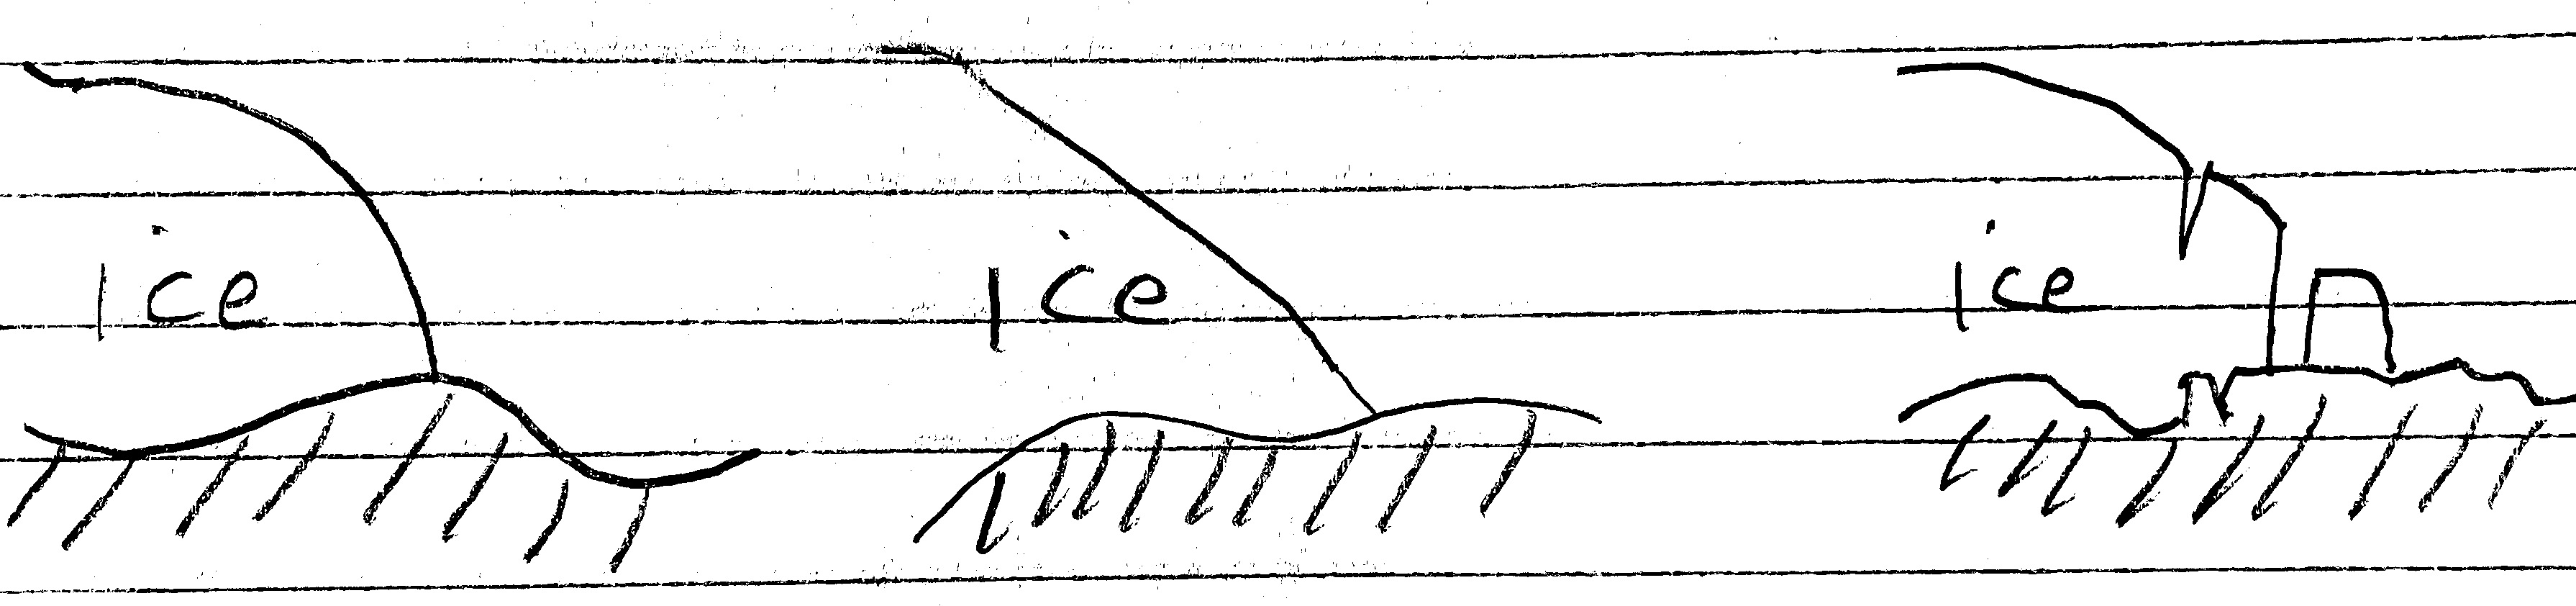
\includegraphics[width=0.8\textwidth]{figs/margins.jpg}
\end{center}
\caption{In which Sobolev space should we seek the surface elevation function?  This question relates to the theoretically-expected shape of the ice margin.  The shallow ice theory yields a fractional power shape (left).  Other glacier models hypothesize a ``wedge'' shape (center).  On the other hand, actual glacier margins often have overhangs, crevasses, and cliffs (right).}
\label{fig:margins}
\end{figure}

Because margins are small features compared to the overall scale of glaciers and ice sheets, almost all modeling literature ignores overhangs and assumes instead that surface and bed elevation functions are well-defined; see \cite{IsaacStadlerGhattas2015,Jouvetetal2008,LofgrenAhlkronaHelanow2022,WirbelJarosch2020} among many examples.  Extending Stokes-based viscous models by allowing overhangs, and supplementing the momentum conservation model with an additional advected damage variable \cite{PralongFunk2005}, so that ice-cliff calving can occur via a stress-failure criterion, might provide a mechanism to explain how (nearly) well-defined surface elevation and thickness functions arise as solutions to the kind of models considered in this paper.

\subsection{Conjectural well-posedness for the continuum problem} \label{subsec:conjecture} Subsections \ref{subsec:noflow}--\ref{subsec:margin} have deployed various imperfect arguments to explain why the backward Euler VI problem \eqref{eq:be:vi} could be well-posed, or at least why other approaches are less promising.  We now state a mathematically-precise conjectural framework for well-posedness of this problem based upon the idea that the surface motion map $\Phi(s) = -\bu|_s\cdot \bn_s$ assigns significantly different results to inputs which are different in norm.

\begin{conjecture} \label{conj:b}  For $\rr>2$ such that Conjecture \ref{conj:a} holds, let $\cX = W^{1,\rr}(\Omega)$.  Fix $b\in\cX$ and let $\cK=\{r\in\cX\,:\,r\ge b\}$.  Recall $\Phi:\cK\to\cX'$ is then well-defined by Lemma \ref{lem:philipschitz}.  Then there are constants $\alpha>0$ and $\qq>1$ so that
\begin{equation}
\left(\Phi(r) - \Phi(s)\right)[r-s] \ge \alpha \|r-s\|_{\cX}^\qq \qquad \text{for all } r,s\in\cK. \label{eq:conj:b}
\end{equation}
\end{conjecture}

In Section \ref{sec:abstractestimate}, inequality \eqref{eq:conj:b} will be called $\qq$-\emph{coercivity} of $\Phi$ over $\cK$.  In the abstract VI context of that Section, if $F_{\Delta t}$ is both Lipschitz continuous (Lemma \ref{lem:philipschitz}) and $\qq$-coercive, over a closed and convex subset $\cK$ of a Banach space $\cX$, then \eqref{eq:be:vi} is well-posed.  This is what we prove next, namely that Conjectures \ref{conj:a} and \ref{conj:b} are sufficient for well-posedness of each implicit time step VI problem \eqref{eq:be:vi}.

\begin{theorem} \label{thm:stepwellposed}  Assume Conjectures \ref{conj:a} and \ref{conj:b}, and fix $b \in \cX$ to define $\cK$.  Suppose that $s^{n-1}\in\cK$ and that the SMB function $a(t,x)$ is in $C([0,T]; L^{\rr'}(\Omega))$.  Then there exists a unique surface elevation $s\in\cK$ satisfying backwards Euler VI problem \eqref{eq:be:vi}. \end{theorem}

\begin{proof}  Let $\rho>0$.  By Lemma \ref{lem:philipschitz} there is $C(\rho)>0$ so that if $r,s\in B_\rho\cap\cK$ then $\big|\Phi(r)[q] - \Phi(s)[q]\big| \le C(\rho) \|r-s\|_{\cX} \|q\|_{\cX}$.  Then by definition \eqref{eq:be:Fdefine}, H\"older's inequality, and Sobolev's inequality we have
\begin{align}
\left|F_{\Delta t}(r)[q] - F_{\Delta t}(s)[q]\right| &\le \int_\Omega |r-s||q| + \Delta t\, \big|\Phi(r)[q] - \Phi(s)[q]\big| \\
    &\le C(\rho,\Delta t) \|r-s\|_{\cX} \|q\|_\cX. \notag
\end{align}
Thus $F_{\Delta t}$ is also (Lipschitz) continuous on bounded subsets of $\cK$.  If $\Delta t>0$ and \eqref{eq:conj:b} holds then
\begin{align}
\left(F_{\Delta t}(r) - F_{\Delta t}(s)\right)[r-s] &= \int_\Omega (r-s)^2 + \Delta t\, \left(\Phi(r) - \Phi(s)\right)[r-s] \\
    &\ge \alpha\Delta t \|r-s\|_{\cX}^\qq, \notag
\end{align}
so $F_{\Delta t}$ is $\qq$-coercive over $\cX$.  Let $q\in\cX$.  From definition \eqref{eq:be:source}, the hypothesis on $a$, and H\"older's inequality,
\begin{equation}
\big|\ell^n[q]\big| \le \left(\|s^{n-1}\|_{L^{\rr'}} + \Delta t \max_{t\in[t_{n-1},t_n]} \|a(t,\cdot)\|_{L^{\rr'}}\right) \|q\|_{L^\rr}.
\label{eq:sourcetermbound}
\end{equation}
Because $\|s^{n-1}\|_{L^{\rr'}}$ is finite by Sobolev's inequality, and because $\|q\|_{L^\rr} \le \|q\|_{\cX}$, it follows that the source term $\ell^n$ is in the dual space $\cX'$.

As noted below in Section \ref{sec:abstractestimate}, because $F_{\Delta t}$ is $\qq$-coercive it is also coercive and strictly-monotone.  Now Corollary III.1.8 of \cite{KinderlehrerStampacchia1980} shows existence of a solution to \eqref{eq:be:vi}, which is unique by strict monotonicity.
\end{proof}

Theorem \ref{thm:stepwellposed} addresses the well-posedness of a single time-step problem over $[t_{n-1},t_n]$.  Its conclusion is not sufficient to show well-posedness of the time-dependent problem parabolic VI problem, over $[0,T]$, corresponding to NCP \eqref{eq:ncp}.  If this problem were known to be well-posed then one might analyze whether implicit steps converge in the $\Delta t\to 0$ limit.

It would seem that those modeling practitioners who use Stokes dynamics expect Conjectures \ref{conj:a} and \ref{conj:b}, or equivalents, to hold, but they may be difficult to prove despite some progress in Sections \ref{sec:stokes} and \ref{sec:model}.  Greater progress which has been made in the SIA case \cite{Calvoetal2003,JouvetBueler2012,PiersantiTemam2023}, which might be helpful.

The computation of $\bu|_s$ and $\Phi(s)=-\bu|_s\cdot \bn_s$, or equivalent expressions, would seem to be necessary in any evolving-geometry Stokes framework, and only these expressions are addressed in the Conjectures.  By contrast, the backward Euler scheme used here is merely the simplest A-stable \cite{AscherPetzold1998} scheme which can be applied.  (Note that for finite dimensional DAE problems, implicit and A-stable schemes are standard \cite{AscherPetzold1998}.)  In any case, the geometry error bounds and results in the next two Sections only require Theorem \ref{thm:stepwellposed}.


\section{Abstract error estimate for a finite element approximation} \label{sec:abstractestimate}

We now consider the finite element (FE) approximation of an abstract variational inequality (VI) problem.  We will return to the glaciological problem \eqref{eq:be:vi} in Section \ref{sec:application}.

Let $\cX$ be a real reflexive Banach space with norm $\|\cdot\|$ and topological dual space $\cX'$.  Denote the dual pairing of $\ell \in \cX'$ and $v\in\cX$ by $\ell[v]$, and define the (Banach space) norm on $\cX'$ by $\|\phi\|_{\cX'} = \sup_{\|v\|=1} \big|\ell[v]\big|$.  Let $\cK \subset \cX$ be a nonempty, closed, and convex subset.  It is called the constraint set, and its elements are said to be admissible.

For a continuous, but generally nonlinear, operator $f:\cK \to \cX'$, and a linear source $\ell\in \cX'$, the VI problem is to find $u\in \cK$ such that
\begin{equation}
f(u)[v-u] \ge \ell[v-u] \quad \text{for all } v\in \cK. \label{eq:vi}
\end{equation}
The best known example of such a problem is the obstacle problem for the Laplacian operator; see \cite{Ciarlet2002,Evans2010,KinderlehrerStampacchia1980} for its theory and FE analysis.

The following definitions are standard \cite[Chapter III]{KinderlehrerStampacchia1980}.  The definition of $\qq$-coercive has already appeared in Conjecture \ref{conj:b}.

\begin{definition} \label{def:monotonecoercive}
An operator $f:\cK \to \cX'$ is said to be \emph{monotone} if
\begin{equation}
\left(f(v)-f(w)\right)[v-w] \ge 0 \qquad \text{for all } v,w \in \cK \label{eq:monotone}
\end{equation}
and \emph{strictly monotone} if equality in \eqref{eq:monotone} implies $v=w$.  It is \emph{coercive} if there is $w\in \cK$ so that
\begin{equation}
\frac{\left(f(v)-f(w)\right)[v-w]}{\|v-w\|} \to +\infty \qquad \text{for } v \in \cK \text{ as } \|v\| \to +\infty. \label{eq:coercive}
\end{equation}
Let $\qq>1$.  The operator is \emph{$\qq$-coercive \cite{Bueler2021conservation}} if there exists $\alpha>0$ such that
\begin{equation}
\left(f(v)-f(w)\right)[v-w] \ge \alpha \|v-w\|^\qq \qquad \text{for all } v,w \in \cK. \label{eq:qcoercive}
\end{equation}
\end{definition}

If $f:\cK \to \cX'$ is monotone and coercive, and also continuous on finite-dimensional subspaces, then VI \eqref{eq:vi} has a solution \cite[Corollary III.1.8]{KinderlehrerStampacchia1980}.  If $f$ is strictly monotone then the solution is unique.  If $f$ is $\qq$-coercive then it coercive and strictly monotone, so $\qq$-coercivity and continuity yield well-posedness for \eqref{eq:vi}.
% \cite{Peral1997} uniform continuity over bounded sets for p-Laplacian: Thm A.0.6

The following definition appeared in Lemma \ref{lem:philipschitz}.  Note that Definitions \ref{def:monotonecoercive} and \ref{def:lipshitz} do not require $f$ to be defined on all of the vector space $\cX$, but only on $\cK$.  If Definition \ref{def:lipshitz} applies then $f$ is continuous.

\begin{definition} \label{def:lipshitz}
For $\rho>0$ let $B_\rho = \{v\in \cX\,:\,\|v\|\le \rho\}$.  We say $f:\cK \to \cX'$ is \emph{Lipshitz on bounded subsets of $\cK$} if for every $\rho>0$ there is $C(\rho)>0$ so that if $v,w \in B_\rho \cap \cK$ and $z\in\cX$ then $|\left(f(v)-f(w)\right)[z]| \le C(\rho) \|v-w\| \|z\|$, equivalently
\begin{equation}
\|f(v)-f(w)\|_{\cX'} \le C(\rho) \|v-w\| \quad \text{ for all } v,w \in B_\rho \cap \cK.  \label{eq:liponbounded}
\end{equation}
\end{definition}

A key concept in the following theorem is that $f(u)-\ell \in \cX'$ is generally nonzero when $u$ solves \eqref{eq:vi}.  An NCP like \eqref{eq:ncp} or \eqref{eq:be:ncp} holds, at least in sufficiently regular cases, but only for $u$ in the interior of $\cK$ should we expect equality $f(u)=\ell$.
%See \cite[Exercise 5.1.1]{Ciarlet2002} and \cite[section 7]{BuelerFarrell2024} for examples.

An FE method for \eqref{eq:vi} is a finite-dimensional VI problem.  Suppose $\cX_h \subset \cX$ is a finite-dimensional subspace; typically $\cX_h$ consists of continuous, piecewise-polynomial functions defined on a mesh.  The FE constraint set $\cK_h\subset \cX_h$ is closed and convex, but generally $\cK_h \nsubseteq \cK$.  Let $f_h:\cK_h\to\cX'$, and note that generally $f_h\ne f$ because of quadrature and other approximations.  The FE VI problem is
\begin{equation}
f_h(u_h)[v_h-u_h] \ge \ell[v_h-u_h] \quad \text{for all } v_h\in \cK_h. \label{eq:fe:vi}
\end{equation}
We will assume that this FE problem is well-posed, so that it uniquely defines $u_h\in\cK_h$, but we will not need to assume specifically that $f_h$ is $\qq$-coercive, Lipschitz, or even continuous.

The following abstract error estimate extends \cite{Falk1974} and Theorem 5.1.1 in \cite{Ciarlet2002}.  Here we do not assume that $f$ is linear, nor that $\cK_h \subset \cK$ or $f_h=f$.  Also, $f_h$ needs only be defined on $\cK_h$.  However, we must extend the domain of $f$ to include the FE solution.

\begin{theorem} \label{thm:abstractestimate}  Suppose $u\in\cK$ solves \eqref{eq:vi} and $u_h\in\cK_h$ solves \eqref{eq:fe:vi}.  Define
\begin{equation}
\hcK = \overline{\Hull{(\cK \cup \cK_h)}}  \label{eq:convexhull}
\end{equation}
as the closure in $\cX$ of the convex hull of $\cK \cup \cK_h$, and suppose that $f$ can be extended to $\hcK$.  For $\qq>1$, with conjugate $\qq'=\qq/(\qq-1)$, assume that $f$ is $\qq$-coercive over $\hcK$ with constant $\alpha>0$, and Lipshitz on bounded sets of $\hcK$.  Let $R_h=\max\{\|u\|,\|u_h\|\}$.  Then there is a constant $c=c(\alpha,R_h)>0$, which does not otherwise depend on $u$ or $u_h$, so that
\begin{align}
\|u-u_h\|^\qq &\le \quad \frac{2}{\alpha} \inf_{v\in\cK} \left(f(u)-\ell\right)[v-u_h] \label{eq:abstractestimate} \\
   &\quad\, + \frac{2}{\alpha} \inf_{v_h\in\cK_h} \left(f(u)-\ell\right)[v_h-u] \notag \\
   &\quad\, + \frac{2}{\alpha} \left(f(u_h)-f_h(u_h)\right)[u_h] \notag \\
   &\quad\, + \inf_{v_h\in\cK_h} c \|v_h - u\|^{\qq'} \notag
\end{align}
\end{theorem}

\begin{proof}  For arbitrary $v\in\cK$ and $v_h\in\cK_h$, rewrite \eqref{eq:vi} and \eqref{eq:fe:vi} as follows:
\begin{align*}
f(u)[u]     &\le f(u)[v] + \ell[u-v],  \\
f_h(u_h)[u_h] &\le f_h(u_h)[v_h] + \ell[u_h-v_h].
\end{align*}
It follows from $\qq$-coercivity of $f$, and these inequalities, that
\begin{align*}
\alpha \|u-u_h\|^\qq &\le \left(f(u)-f(u_h)\right)[u-u_h] \\
  &= f(u)[u] + f(u_h)[u_h] - f(u)[u_h] - f(u_h)[u] \\
  &= f(u)[u] + f_h(u_h)[u_h] \\
  &\qquad - f(u)[u_h] - f(u_h)[u] + \left(f(u_h)-f_h(u_h)\right)[u_h] \\
  &\le f(u)[v] + \ell[u-v] + f(u_h)[v_h] + \ell[u_h-v_h] \\
  &\qquad - f(u)[u_h] - f(u_h)[u] + \left(f(u_h)-f_h(u_h)\right)[u_h] \\
  &= f(u)[v-u_h] - \ell[v-u_h] + f(u_h)[v_h-u] - \ell[v_h-u] \\
  &\qquad + \left(f(u_h)-f_h(u_h)\right)[u_h] \\
  &= \left(f(u)-\ell\right)[v-u_h] + \left(f(u)-\ell\right)[v_h-u] \\
  &\qquad + \left(f(u)-f(u_h)\right)[u-v_h] + \left(f(u_h)-f_h(u_h)\right)[u_h]
\end{align*}
Since $u,u_h\in B_{R_h}$, by the Lipshitz assumption over $\hcK$ there is $C(R_h)>0$ so that
    $$\left(f(u)-f(u_h)\right)[u-v_h] \le C(R_h) \|u-u_h\|\|u-v_h\|.$$
Noting $1<\qq<\infty$, now use Young's inequality with $\eps>0$ \cite[Appendix B.2]{Evans2010}:
\begin{align*}
\alpha \|u-u_h\|^\qq &\le \left(f(u)-\ell\right)[v-u_h] + \left(f(u)-\ell\right)[v_h-u] \\
  &\qquad + C(R_h) \left(\eps\|u-u_h\|^\qq + \tilde C(\eps) \|u-v_h\|^{\qq'}\right) + \left(f(u_h)-f_h(u_h)\right)[u_h],
\end{align*}
where $\tilde C(\eps) = (\eps \qq)^{-\qq'/\qq} {\qq'}^{-1}$.  Choose $\eps>0$ so that $C(R_h) \eps \le \alpha/2$, and subtract:
\begin{align*}
\frac{\alpha}{2} \|u-u_h\|^\qq &\le \left(f(u)-\ell\right)[v-u_h] + \left(f(u)-\ell\right)[v_h-u] \\
  &\qquad + C(R_h) \tilde C(\eps) \|u-v_h\|^{\qq'} + \left(f(u_h)-f_h(u_h)\right)[u_h]
\end{align*}
Take infimums to show \eqref{eq:abstractestimate}.
\end{proof}

There are two important cases where the essentially-technical convex hull operation \eqref{eq:convexhull} is not needed.  We will see in Section \ref{sec:application} that case \emph{i)} can be practically arranged in glacier simulations.

\begin{corollary}  \label{cor:abstractestimate:nohull}  In addition to the assumptions of Theorem \ref{thm:abstractestimate}, suppose that one of the following situations apply:
\renewcommand{\labelenumi}{\roman{enumi})}
\begin{enumerate}
\item $\cK_h \subset \cK$, with $f$ being $\qq$-coercive over $\cK$, or
\item $f$ is defined on, and $\qq$-coercive over, all of $\cX$.
\end{enumerate}
Then, without the construction of the convex hull $\hcK$, conclusion \eqref{eq:abstractestimate} applies as stated, except that in case i) the ``\,$\inf_{v\in\cK}$'' term is zero.
\end{corollary}

Consider $f(u)-\ell\in \cX'$ in Theorem \ref{thm:abstractestimate}, which might be a signed measure or a real-valued measurable function.  The first two terms in estimate \eqref{eq:abstractestimate} include information about its sign.  By contrast, the Hilbert space result in \cite{Falk1974} (and \cite[section 5.1]{Ciarlet2002}) computes norms, and loses this information.  The following corollary, with easy proof, takes the norm-based approach.  We suppose that $\cX$ continuously and densely embeds into a larger Banach space $\cB$:
\begin{equation}
\cX \hookrightarrow \cB, \quad \bar{\cX} = \cB \label{eq:VembedsinB}
\end{equation}
Observe that $\cB' \subset \cX'$.  A standard example is $\cX=W^{1,\rr}(\Omega)$ and $\cB=L^\rr(\Omega)$.

\begin{corollary}  \label{cor:abstractestimate:Bnorm}  In addition to the assumptions of Theorem \ref{thm:abstractestimate}, suppose \eqref{eq:VembedsinB} and that $\|f(u)-\ell\|_{\cB'} < \infty$.  Then
\begin{align}
\|u-u_h\|^\qq &\le \frac{2}{\alpha} \|f(u)-\ell\|_{\cB'} \left( \inf_{v\in\cK} \|v-u_h\|_{\cB} +   \inf_{v_h\in\cK_h} \|v_h-u\|_{\cB} \right) \label{eq:abstractestimate:Bnorm} \\
   &\qquad + \frac{2}{\alpha} \left(f(u_h)-f_h(u_h)\right)[u_h] + \inf_{v_h\in\cK_h} c \|v_h - u\|^{\qq'} \notag
\end{align}
\end{corollary}

The result by Falk \cite{Falk1974} combines the above two Corollaries, under the further assumption that $f$ is linear.  Specifically, suppose $f(v)[w]=a(v,w)$ is actually bilinear, uniformly elliptic, and continuous on a Hilbert space $\cX$.  In this bilinear case, the definition of uniformly elliptic coincides with definition \eqref{eq:qcoercive} of $2$-coercive, and continuity of $a(v,w)$ implies Lipshitz on bounded sets \eqref{eq:liponbounded} for $f$.  Suppose that $\cX\hookrightarrow \cH$ and $\bar{\cX} = \cH$ for some Hilbert space $\cH$, and that $\|f(u)-\ell\|_{\cH'} < \infty$ so that, up to isomorphism, $f(u)-\ell \in \cH$.  Finally, suppose that $f(u_h)=f_h(u_h)$.  Then case \emph{ii)} of Corollary \ref{cor:abstractestimate:nohull}, and Corollary \ref{cor:abstractestimate:Bnorm}, reduce to Theorem 1 in \cite{Falk1974}, and also Theorem 5.1.1 in \cite{Ciarlet2002}.

As observed in \cite{Ciarlet2002}, the quantity in estimates \eqref{eq:abstractestimate} and \eqref{eq:abstractestimate:Bnorm} which involves $v-u_h$, for $v\in\cK$, is generally nonzero in obstacle problems where $\cK_h \nsubseteq \cK$.  This observation is important for glacier models tracking the surface elevation, as opposed to thickness.  In fact, consider a unilateral obstacle problem where $\cK=\{v \in \cX\,:\,v\ge \psi\}$.  Suppose $\psi_h$ is an FE interpolant of $\psi$, and $\cK_h=\{v_h \in \cX_h\,:\,v_h\ge \psi_h\}$.  Observe that, while $\psi_h(x_j)=\psi(x_j)$ for interpolation nodes $x_j$, generally $\psi_h(x) \ge \psi(x)$ does not hold for all $x\in\Omega$, even if $\psi$ is arbitrarily smooth.  In other words, nodal admissiblity does not imply admissibility (Figure \ref{fig:nonadmissible}).  However, in Section \ref{sec:application} we will see that a one-sided interpolation process allows us to bypass this concern for glacier models using surface elevation.  Those which solve for ice thickness avoid this concern because then $\cK = \{v\in\cX\,:\,v\ge 0\}$, and generally $\cK_h=\cK\cap\cX_h \subset \cK$.

\begin{figure}[ht]
\begin{center}
FIXME figure like Ciarlet Figure 5.1.3 %\includegraphics[width=0.8\textwidth]{figs/xxx.jpg}
\end{center}
\caption{Nodal admissibility generally does not imply admissibility.  Thus, if $\phi_h$ is the FE interpolant of an obstacle $\psi$, it is possible that $\cK_h \nsubseteq \cK$.}
\label{fig:nonadmissible}
\end{figure}

The following corollary collects various conclusions one may draw from making stronger assumptions, especially that the discretized operator is exact on $u_h$.

\begin{corollary}  \label{cor:abstractestimate:various}  Make the assumptions of case i) of Corollary \ref{cor:abstractestimate:nohull}, including that $\cK_h \subset \cK$.  Also assume that $f_h(u_h)[u_h] = f(u_h)[u_h]$.  Then
\begin{equation}
\|u-u_h\|^\qq \le  \inf_{v_h\in\cK_h} \left\{\frac{2}{\alpha} \left(f(u)-\ell\right)[v_h-u] + c \|v_h - u\|^{\qq'}\right\}. \label{eq:abstractestimate:subset}
\end{equation}
If also the assumptions of Corollary \ref{cor:abstractestimate:Bnorm} hold then
\begin{equation}
\|u-u_h\|^\qq \le \inf_{v_h\in\cK_h} \left\{\frac{2}{\alpha} \|f(u)-\ell\|_{\cB'} \|v_h-u\|_{\cB} + c \|v_h-u\|^{\qq'}\right\} \label{eq:abstractestimate:subset:Bnorm}
\end{equation}
Finally, if additionally $f(u)=\ell$, for example if $u$ is in the interior of $\cK$, then
\begin{equation}
\|u-u_h\| \le \tilde c \inf_{v_h\in\cK_h} \|v_h-u\|^{\qq'-1} \label{eq:abstractestimate:subset:Cea}
\end{equation}
\end{corollary}

Note that \eqref{eq:abstractestimate:subset:Cea} is Cea's lemma \cite[Theorem 2.4.1]{Ciarlet2002} in a Banach space.  This has reduced to the PDE case where there is no active set or free boundary.  In the glacier context, \eqref{eq:abstractestimate:subset:Cea} applies if the entire domain $\Omega$ is covered in ice, and the other assumptions of Corollary \ref{cor:abstractestimate:various} apply.


\section{Application of the theory to glacier models} \label{sec:application}

Now we can synthesize the theory of previous Sections, and apply it to an implicit time step of a glacier simulation which uses Stokes dynamics.  We will combine the well-posedness theory and \emph{a priori} bounds for the glaciological Stokes problem on a fixed domain (Section \ref{sec:stokes}), the conjectural well-posedness theory of the surface elevation VI problem (Sections \ref{sec:model} and \ref{sec:theory}), and the abstract error estimate for finite element (FE) solutions of VIs (Section \ref{sec:abstractestimate}).  This section also gives a precise meaning to the phrase ``conforming FE method'' for an evolving glacier geometry simulation.

The numerical methods considered here solve FE approximations of VI \eqref{eq:be:vi}.  For some chosen finite-dimensional FE subspace $\cX_h\subset \cX$, with a constraint set $\cK_h\subset \cX_h$ (more below), we seek $s_h\in\cK_h$ solving
\begin{equation}
F^h_{\Delta t}(s_h)[r_h-s_h] \ge \ell^n[r_h-s_h] \quad \text{for all } r_h \in \cK_h. \label{eq:fe:be:vi}
\end{equation}
Here $\ell^n = s^{n-1} + \Delta t\,a^n$ is defined as before, by equation \eqref{eq:be:source}.

The operator $F^h_{\Delta t}$ in \eqref{eq:fe:be:vi} denotes an FE approximation to the operator $F_{\Delta t}$, which is defined in \eqref{eq:be:Fdefine}.  As illustrated in Figure \ref{fig:fe:operatorvisualization}, evaluation of $F^h_{\Delta t}(s_h)$ requires the numerical solution of a glaciological Stokes problem \eqref{eq:stokes} for the surface elevation $s_h$, presumably over a 3D mesh generated for the domain $\Lambda=\Lambda_{s_h}$ between $s_h$ and $b_h$.  This numerical result will not produce the exact value $F_{\Delta t}(s_h)$ for the same surface because the trace of the numerical velocity will be only approximate: $\bu_h|_{s_h} \approx \bu|_{s_h}$.

\begin{figure}[ht]
\begin{center}
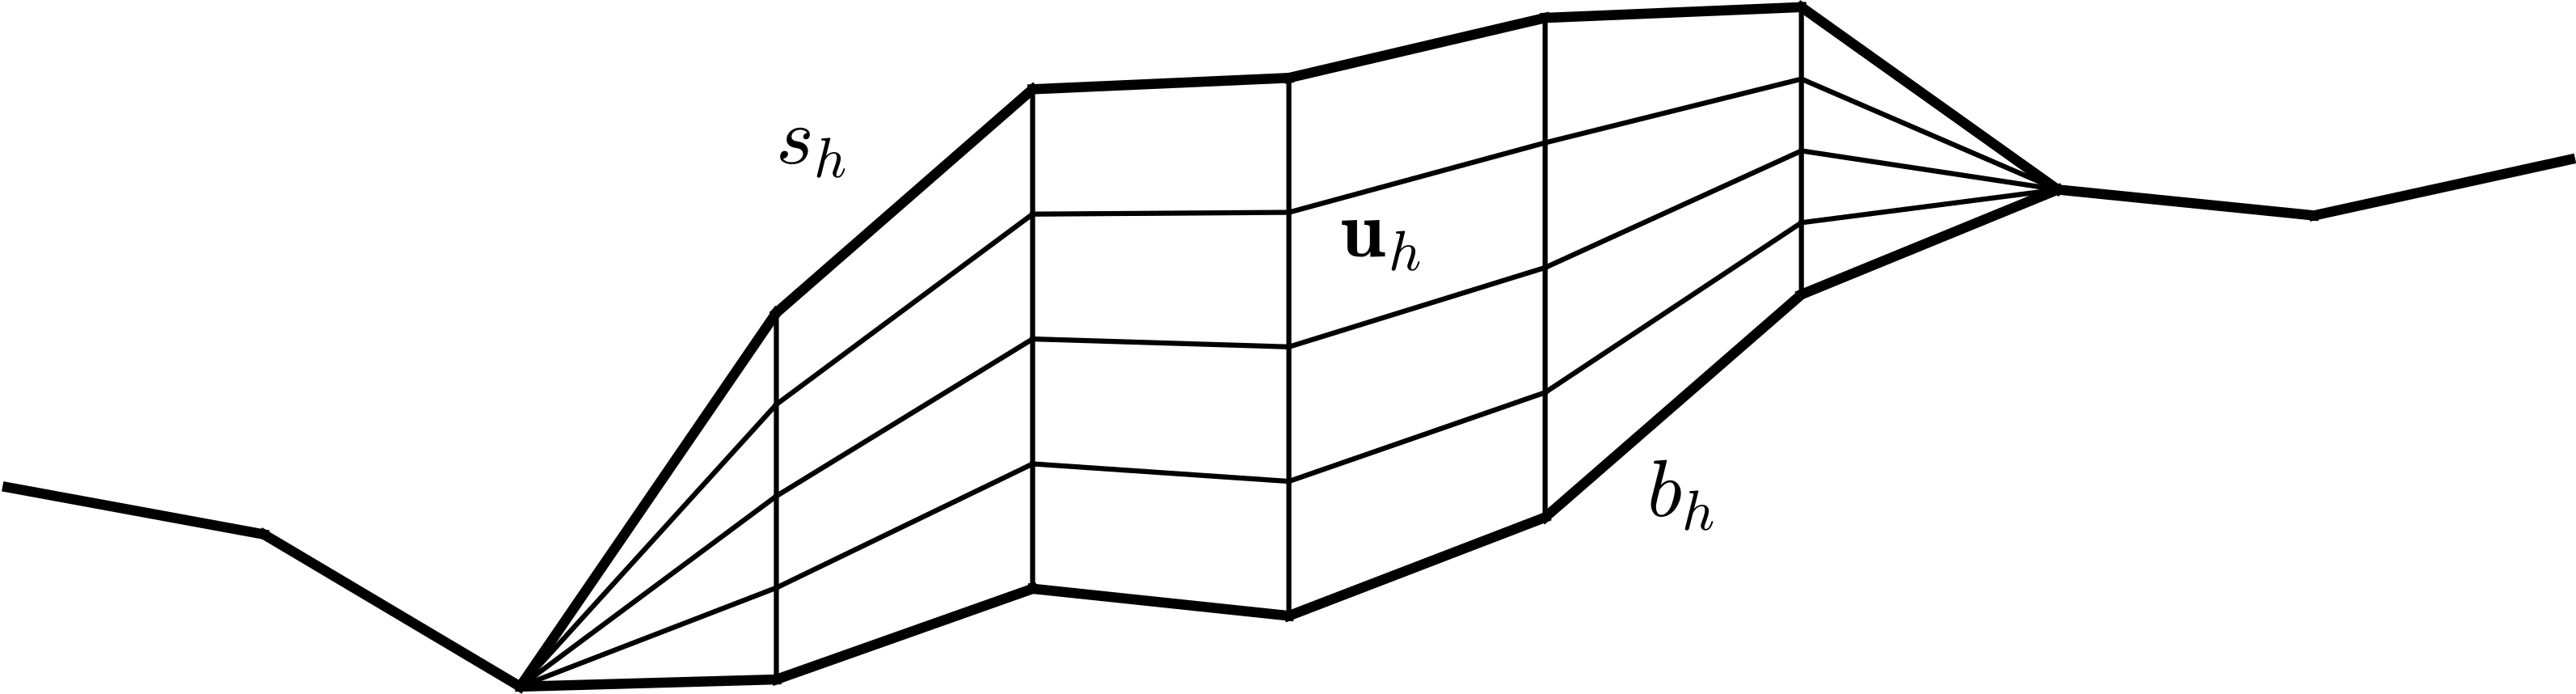
\includegraphics[width=0.55\textwidth]{genfigs/extruded.pdf}
\end{center}
\caption{Evaluating $F^h_{\Delta t}(s_h)$ in the numerical free-boundary problem \eqref{eq:fe:be:vi} requires numerically solving a Stokes problem on a mesh like this, then evaluating the surface trace, on $s_h$, of the solution velocity $\bu_h$.  See formula \eqref{eq:be:Fdefine}.}
\label{fig:fe:operatorvisualization}
\end{figure}

A key concern in applying Theorem \ref{thm:abstractestimate}, or its Corollaries, is the choice of the numerical bed elevation $b_h \approx b\in\cX$, needed to construct the constraint set $\cK_h$.  In the glaciological context one may assume $b$ is continuous on the closed domain $\bar\Omega$.  An abstract $b\in C(\bar\Omega) \cap \cX$ can be considered, but in practice $b$ will be provided via a high resolution map derived from e.g.~ice-penetrating radar \cite{Morlighemetal2017}.  In the following we are asserting that $b_h \in \cX_h$ with $b_h\ge b$ should be chosen; the results demonstrate why this is a good choice.  To achieve $b_h\ge b$, maximum monotone restriction \cite{BuelerFarrell2024} or similar can be applied, that is, $b_h = R^\oplus b$ or $b_h = (R^\oplus)^k b$, at least if $\cX_h$ is from a submesh of the data mesh.  We will also assume that $b|_{\partial\Omega}$ is piecewise-polynomial, to allow ``conforming'' in the classical sense \cite{Elmanetal2014}.

From now on we make these standard assumptions.

\smallskip
\begin{assumptions}
The following data are given:
\begin{enumerate}
\item A bounded, convex polygon $\Omega\subset\RR^2$.
\item An exponent $\rr > 2$, with conjugate exponent $\rr' = \rr/(\rr-1)$. \label{item:rr}
\item A time-dependent SMB function $a\in C([0,T]; L^{\rr'}(\Omega))$.
\item A bed topography $b \in C(\bar\Omega) \cap W^{1,\rr}(\Omega)$, with piecewise-polynomial boundary values $b|_{\partial\Omega}$.
\end{enumerate}
We make these definitions:
\begin{enumerate}
\setcounter{enumi}{4}
\item $\cX = W^{1,\rr}(\Omega)$.
\item $\cK = \{r\in\cX\,:\,r|_{\partial \Omega} = b|_{\partial \Omega} \text{ and } r \ge b\}$.
\item $\cX_h \subset \cX$ is a finite-dimensional, conforming FE space, from a mesh over $\bar\Omega$ such that the boundary values $b|_{\partial\Omega}$ are exactly represented.
\end{enumerate}
The following are assumed to hold, for the $\rr > 2$ given in item \emph{\ref{item:rr}}:
\begin{enumerate}
\setcounter{enumi}{7}
\item Conjecture \ref{conj:a} holds with Lipschitz constant $\CA > 0$.
\item Conjecture \ref{conj:b} holds with exponent $\qq>1$ and coercivity constant $\alpha > 0$.
\end{enumerate}
We also assume and define:
\begin{enumerate}
\setcounter{enumi}{9}
\item $b_h\in\cX_h$ is given, with $b_h\ge b$ on $\bar\Omega$ and $b_h|_{\partial \Omega} = b|_{\partial \Omega}$. \label{item:goodbh}
\item $\cK_h = \{r_h\in\cX_h\,:\,r_h|_{\partial \Omega} = b_h|_{\partial \Omega} \text{ and } r_h \ge b_h\}$. \label{item:defineKh}
\end{enumerate}
\end{assumptions}

\medskip
We will see the advantages which follow from the conforming condition $\cK_h\subset \cK$, which follows from assumptions \ref{item:goodbh} and \ref{item:defineKh}.  Applying Corollary \ref{cor:abstractestimate:nohull}, we get the following Lemma.  Note here that $s_h\in\cK$.  Also note that $F_{\Delta t}$ is $\qq$-coercive and Lipschitz on bounded subsets, over $\cK$, as shown in the proof of Theorem \ref{thm:stepwellposed}.

\begin{lemma} \label{lem:preglacierapp}  Make the Standard Assumptions.  Suppose that $s^{n-1}\in\cK$ and define $\ell^n \in \cX'$ by \eqref{eq:be:source}.  Let $s\in\cK$ be the unique surface elevation satisfying the continuum implicit time-step VI problem \eqref{eq:be:vi}, the result of Theorem \ref{thm:stepwellposed}.  Assume $F^h_{\Delta t}$ represents a numerical scheme for the FE VI problem \eqref{eq:fe:be:vi}, and let $s_h\in\cK_h$ be a solution of \eqref{eq:fe:be:vi}.  Let $R_h=\max\{\|s\|_\cX,\|s_h\|_\cX\}$.  Then there is a constant $c=c(R_h)>0$, not otherwise depending on $s$ or $s_h$, so that
\begin{align}
\|s-s_h\|_\cX^\rr &\le \quad \frac{2}{\alpha} \inf_{r_h\in\cK_h} \left(F_{\Delta t}(s)-\ell^n\right)[r_h-s] \label{eq:glacierestimate} \\
   &\quad\, + \frac{2}{\alpha} \left(F_{\Delta t}(s_h)-F^h_{\Delta t}(s_h)\right)[s_h] \notag \\
   &\quad\, + \inf_{r_h\in\cK_h} c \|r_h - s\|_{\cX}^\qq \notag
\end{align}
\end{lemma}

\begin{proof}
A straightforward application of Corollary \ref{cor:abstractestimate:nohull} in case \emph{i)}.
\end{proof}

FIXME generate a full theorem from the Lemma

FIXME accomodate the barrier theory from \cite{Bueler2021conservation}


\section{Demonstration in a numerical glacier model} \label{sec:demo}

FIXME study 2D glaciers with Halfar-ish surfaces and 3 bed cases: flat, smooth, rough

FIXME for pairs of states generated in this study also compute ratios
\begin{equation}
\frac{\big\|\bu|_r - \bu|_s\big\|_{L^{\rr'}}}{\|r-s\|_{W^{1,\rr}}} \qquad \text{and} \qquad \frac{\left(\Phi(r) - \Phi(s)\right)[r-s]}{\|r-s\|_{W^{1,\rr}}^\qq}
\end{equation}
to evaluate Conjectures \ref{conj:a} and \ref{conj:b}; presumably use $\rr=\rr'=\qq=2$


\section{Discussion and conclusion} \label{sec:conclusion}

FIXME the following version of Conjecture \ref{conj:b} does not address the marginal overhang issue, and it is likely to be easier to profe, but it is not sufficient for Theorem \ref{thm:stepwellposed}
\begin{conjecture} \label{conj:c}  For $\rr>2$ such that Conjecture \ref{conj:a} holds, let $\cX = W^{1,\rr}(\Omega)$.  Fix $b\in\cX$, let $\cK=\{r\in\cX\,:\,r\ge b\}$, and assume $s\in \cK$.  Then there are constants $\alpha>0$, $\qq>1$, $\delta>0$ so that for all $\psi\in\cX$ supported in the inactive set of $s$, namely $\{x\in\Omega\,:\,s(x)>b(x)\}$, such that $s+\psi\in\cK$ and $\|\psi\|_\cX \le \delta$, the following inequality holds:
\begin{equation}
\left(\Phi(s+\psi) - \Phi(s)\right)[\psi] \ge \alpha \|\psi\|_{\cX}^\qq. \label{eq:conj:c}
\end{equation}
\end{conjecture}

FIXME


\bibliographystyle{siamplain}
\bibliography{estimate}

\end{document}
